\documentclass[twoside]{article}

\usepackage{aistats2019}
\usepackage{amssymb}
\usepackage{graphicx}
% If your paper is accepted, change the options for the package
% aistats2019 as follows:
%
%\usepackage[accepted]{aistats2019}
%
% This option will print headings for the title of your paper and
% headings for the authors names, plus a copyright note at the end of
% the first column of the first page.

% If you set papersize explicitly, activate the following three lines:
%\special{papersize = 8.5in, 11in}
%\setlength{\pdfpageheight}{11in}
%\setlength{\pdfpagewidth}{8.5in}

% If you use natbib package, activate the following three lines:
\usepackage[round]{natbib}
\renewcommand{\bibname}{References}
\renewcommand{\bibsection}{\subsubsection*{\bibname}}

% If you use BibTeX in apalike style, activate the following line:
\bibliographystyle{apalike}
\begin{document}

% If your paper is accepted and the title of your paper is very long,
% the style will print as headings an error message. Use the following
% command to supply a shorter title of your paper so that it can be
% used as headings.
%
%\runningtitle{I use this title instead because the last one was very long}

% If your paper is accepted and the number of authors is large, the
% style will print as headings an error message. Use the following
% command to supply a shorter version of the authors names so that
% they can be used as headings (for example, use only the surnames)
%
%\runningauthor{Surname 1, Surname 2, Surname 3, ...., Surname n}

\twocolumn[

\aistatstitle{Causal Dynamic Time Lag: Predicting What \& When}

\aistatsauthor{Anonymous}

\aistatsaddress{Anonymous} ]

\begin{abstract}
  We formalize the joint regression task of predicting the magnitude of signals as well as the time delay with respect to their driving phenomena. We call the problem \emph{causal dynamic time lag} (CDT), to take note of the non-stationary time delay between the occurrence of causes/drivers and the observation of effects in physical and man-made systems. We propose a solution to the CDT problem and a methodology to benchmark and evaluate causal time lag estimation algorithms.
\end{abstract}

\section{Introduction}
Exploiting causal relationship between time series is a problem of practical importance with many domains of application. Of similar importance is causal relationship between processes. Although rigorous understanding and identification of causal links between arbitrary quantities is an elusive question, for certain situations it is well known that some causal relationship must exist. 

Some of the seminal work relating to causality in time series data is found in \cite{Granger}, which introduced the concept of \emph{Granger Causality}. \emph{Granger causality} focused on the problem of predictive causality instead of the philosophical or \emph{true causality}. Although originally formulated for linear causal relationships with no latent variables, it has since been extended for various situations (see \cite{doi:10.1002/9781119945710.ch22} for a review).

In temporal phenomena, it is also the case that causal effects of events are not immediately observed, but after a certain time interval which can be dynamic. One prominent example of such behavior is the Sun-Earth system and its associated problem of space weather forecasting.

The Sun, a perennial source of charged energetic particles ejects them into the surrounding space. This particle cloud or \emph{solar wind} reaches the Earth's vicinity and interacts with its magnetic field in complex ways, giving rise to geomagnetic phenomena. High speed solar wind can potentially cause damage to under sea pipelines, satellites, and other telecommunication infrastructure. A key prediction task is to forecast  the speed of the \emph{solar wind} in the vicinity of the Earth from solar image data (\cite{doi:10.1002/jgra.50429}, \cite{doi:10.1029/2009SW000542}).

The \emph{solar wind} forecasting problem can be broken down into two stages. First, the extraction of features from solar images and second, the prediction of time lagged solar wind speed near the Earth. In this work we present progress made on the second part of this problem.
 
To our knowledge, the problem of regression with hidden non-constant time delay, as formulated later in section \ref{sec:formulation} has not been addressed in the machine learning literature. 

Similar type of problems have actually been encountered in the context of financial time series prediction in \cite{ZHOU2006195} for instance. Their approach is a form a dynamical time warping (DTW) which appeared originally in the context of speech recognition~\cite{SakoeShiba1978}. \cite{SignalDiffusion} build on the DTW paradigm and take a Bayesian approach to the temporal alignment problem between time series. However they limit themselves to linear relationships between the input and output time series, assuming in addition slow varying time lags.

The DTW algorithm and its variants are now widely used in time series analysis, but they always assume a predefined cost matrix for the temporal alignment between two time series and they assume the causes $x(t)$ and effects $y(t)$ are of same dimensionality and structure. 

Our work has the following novel characteristics as compared to the DTW paradigm.

\begin{enumerate}
    \item Causes and effects are of different dimensionality. The output time series $y(t)$ is scalar, but its driver $x(t)$ is potentially high dimensional, e.g. vectors, images etc.
    \item We do not make assumptions as made in \cite{ZHOU2006195} and other \emph{dynamic time warping} related works about the time lag function. In our case the time lag can be potentially non smooth.
    \item The relationship between $x(t)$ and $y(t)$ can be potentially non-linear. 
\end{enumerate}


\section{Problem Formulation}\label{sec:formulation}

\emph{Causal Dynamic Time Lag} (CDT) is essentially a regression problem with two tasks. Given two time series, the causes $x(t)$ and the observed effects $y(t)$, the regression model must learn a mapping $f()$ which maps each input pattern $x(t_1)$ to an output $y(t_2)$, and a mapping $g(.)$ which maps the time delay between the input and output patterns $t_2 = t_1 + g(x(t_1))$. This is formally specified in equations below.

\begin{align}
y(t + \Delta(t)) & = f[x(t)]\label{eq:pb1}\\
\Delta(t) & = g[x(t)]\label{eq:pb2} 
\end{align}
with
\[
f: \mathcal{X}  \rightarrow \mathbb{R},\qquad\text{and}\qquad
g: \mathcal{X}  \rightarrow \mathbb{R}^{+},
\]
$t \in \mathbb{R}^{+}$ represents the continuous temporal domain. The input signal $x(t)\in \mathcal{X}$ is possibly high dimensional and contains the hidden cause to the effect $y(t)\in\mathbb{R}$ which is considered as a scalar in this paper. $\Delta(t)\in \mathbb{R}^+$ represents the time delay between cause and effect.

It is important to note some caveats about this causal time lag which make the CDT different from classical time series regression problems.

In practical applications such as the motivating space weather example, $\Delta(t)$ is not recorded explicitly in the data set. This makes model training and evaluation challenging.

One may make certain assumptions on the time warping function $\phi(t) = t + g(x(t))$, in the general formulation of the problem presented here: 

\begin{enumerate}
    \item $\phi(.)$ is assumed to be continuous and bijective.
    \item \cite{ZHOU2006195} enforce further assumptions such as $\phi(t_1) \leq \phi(t_2), \forall t_1 \leq t_2$, which are incorporated via constraints. This approach respects the properties associated with the warping function $\phi(.)$ but increase the computational complexity of the resulting optimization problem.
\end{enumerate}

The second assumption can be restrictive for applications in space physics, where fast moving solar wind can reach the Earth before slow moving solar wind which departed before it. 

Our proposed approach works with discrete analogue of the time series $x(t), y(t)$ and does not explicitly enforce assumptions 1 or 2, but instead tries to learn an estimator which for every input $x(t)$, returns an output and time lag estimation. This enables us to benefit from batch wise stochastic gradient learning methods and make our method scalable to larger data sets\footnote{
Another possible approach which naturally come to mind, consists in to alternatively optimize $f$ and $g$ by using a DTW routine in the loop. This however would be far more expensive and not really scalable to large datasets.}.

\section{Proposed Solution}\label{sec:model}

In practical time-series applications, one works with sub-sampled or discretized versions of the time 
series $x(t)$ and $y(t)$. The time delay function $g(.)$ can now be recast as a function which for every
input pattern $x(t_i)$, returns a time delay $\delta$ corresponding to the time step $t_i + \delta$ when,
the effect $y(t_i + \delta)$ is observed.

For practical purposes one must define for every time step $t$, a \emph{causal time window} $[t+\ell, t+\ell+h)$, within which the model searches for probable temporal causal links. Instead of predicting $\delta \in [\ell, \ell+h)$, one can provide a predictive distribution over the causal time interval.

Our proposed model thus produces for a given input $x(t)$ at time $t$ the following predictions:

\begin{enumerate}
\item Targets $\hat{y}(t+\ell), \cdots, \hat{y}(t+\ell+h-1)$
\item Time Lag Probabilities $\hat{p}(t+\ell), \cdots, \hat{p}(t+\ell+h-1)$
\end{enumerate}

The model thus tries to learn a predictor for each lagged output $y(t+i)$ in the causal window $[t+\ell, t+\ell+h)$, and simultaneously supplies a probability distribution over each time step of the causal window, $\hat{p}(t+i)$.

The distribution $\hat{p}(t+i), i \in {\ell, \cdots, \ell+h-1}$ represents the 
likelihood of a causal link between $x(t)$ and $y(t+i)$. Since the model looks
for causal links in the finite window $[t+\ell, t+\ell+h)$, we have 
$\sum^{\ell+h-1}_{i = \ell}{\hat{p}(t + i)} = 1$.


\section{Loss Function}

In order to train time lag based models, one must balance two incentives.

\begin{enumerate}
    \item Generate accurate predictions for time window $y(t+\ell), \cdots, y(t+\ell+h-1)$
    \item Learn the time lag structure.
\end{enumerate}

These incentives have very different contexts. We have access to measurements of the output time series $y(t)$, but that is generally not the case for the time lag structure. Although it is possible that certain data sets may have patterns annotated with time lag information, this is not the norm.

We express the loss function as a sum of two terms (equation \ref{eq:loss}):
\begin{equation}\label{eq:loss}
\begin{aligned}
\mathcal{L}(y^{(1:M)}, &\hat{y}^{(1:M)}, \hat{p}^{(1:M)}) =\\ 
&\lambda_1 \sum_{i,m}{\frac{1}{2M} (y^{(m)}_{i} - \hat{y}^{(m)}_{i})^2 (1 + \hat{p}^{(m)}_i)} \\ 
+ &\lambda_2 \mathcal{J}(y^{(1:M)}, \hat{y}^{(1:M)}, \hat{p}^{(1:M)}).
\end{aligned}
\end{equation}

The above loss function is computed over a mini-batch of size $M$, the indices $i$ denote the
individual components of each prediction, while $m$ refers to data sample indices within the
mini-batch in question.

The first term, weighted with parameter $\lambda_1$ involves a weighted $L_2$ 
error between the predictions $\hat{y}^{(m)}_{i}$ and the targets $y^{(m)}_{i}$. The second term, weighted with parameter $\lambda_2$ has to penalize the predicted probabilities $\hat{p}^{(m)}$ in a meaningful manner. This can be done by considering some \emph{target probability} and calculating some distance/divergence from such a target.

\subsection{Weighted Error}

We want to avoid the situation where the model cherry picks one of the outputs $j$ in the causal time window and concentrates most of the predictive distribution $\hat p^{(m)}$ around the time index $j$. 
The factor $(1+\hat p_i^{(m)})$ instead of $\hat p_i^{(m)}$ in the first term contributes 
to avoid this cherry picking effect. It forces the model to generate well performing
predictions for the entire causal window and then move its predictive distribution
to peak around the most predictable time index.

\subsection{Target Probability}

Let us specify now the second term of the loss function.
From the intuitions of Granger causality, we use the concept of causality as predictability, we can thus characterize the \emph{target probability}, $\widetilde{p}$ for a time window $[t+\ell, t+\ell+h)$ in the following manner: The lagged output $y(t+i)$ which has greater predictability given $x(t)$, is a more likely causal link. This idea is represented in equation \ref{eq:targetprob}, by means of the softmax function and a smoothing parameter $\beta$.

\begin{equation}\label{eq:targetprob}
\widetilde{p}_{i}^{(m)} = \frac{exp \left(- \beta (y_{i}^{(m)} - \hat{y}_{i}^{(m)})^{2} \right)}{\sum_{i}{exp \left(- \beta (y_{i}^{(m)} - \hat{y}_{i}^{(m)})^{2} \right)}} 
\end{equation}

The hyper-parameter $\beta$ serves to determine how sharp the target probability distribution is around its peak. The predictions $\hat{y}^{(m)}_{i}$, made by the model are penalized for their divergence from the \emph{target probability} via the \emph{Hellinger distance} metric (equation \ref{eq:hellinger}).

\begin{align}\label{eq:prior}
& \mathcal{J}(y^{(1:M)}, \hat{y}^{(1:M)}, \hat{p}^{(1:M)}) = \sum_{m = 1}^{M}{\frac{1}{M} \mathcal{H}(\hat{p}^{(m)}, \widetilde{p}^{(m)})} \\
& \mathcal{H}(p, q) = \sqrt{\sum_{i}{(\sqrt{p_i} -  \sqrt{q_i})^2}} \label{eq:hellinger}
\end{align}

There are a number of candidate choices for defining the model's divergence from the \emph{target probability}, i.e.  \emph{Kullback-Leibler divergence} (\cite{kullback1951}), \emph{Jensen-Shannon divergence} (\cite{jensen-shannon}), \emph{Total Variational distance} (\cite{Villani2009}), \emph{Hellinger distance} (\cite{hellinger}) and \emph{Bhattacharya distance} (\cite{bhattacharyya}) to name a few. We found that for the applications considered in this work, \emph{Hellinger distance} worked best. In principle it is possible to use any one of the mentioned divergence/distance measures as a penalty, since the work outlined in this paper is general in nature.

\subsection{Hyper-parameters}

The quantities $\lambda_1, \lambda_2, \beta$ are hyper-parameters which must be adjusted to the application at hand.

The weights $\lambda_1, \lambda_2$ control the importance of each term in the loss (equation \ref{eq:loss}).

The choice of $\beta$ is generally empirical and depends on two criteria 
\begin{enumerate} \item The size of the causal window, $\beta$ should decrease with increasing causal window $h$. 
\item Sharpness/Confidence of the predictive distribution, as $\beta$ increases, the \emph{target} probability distribution tends to be more peaked.  \end{enumerate}

Care must be taken to not set $\beta$ to a value that is very large ($\gg 1$), as this may cause numerical instabilities in the learning/optimization process. 

After some trial and error adjusting the values of the hyper-parameters, we settled on the values $\beta = \frac{4}{3}, \lambda_1 = 1, \lambda_2 = 0.85$ which worked adequately for the experiments in section \ref{sec:exp}.

\section{Model Architecture}

The choice of model architecture is constrained by only one condition, i.e. the number of neurons in the output layer must be $2 \times h$ where $h$ is the chosen size of the causal window. The composition and size of the layers preceding the output layer are dependent on the application, one may choose \emph{convolutional layers} for input data which consists of images and fully connected layers for vector data.

\begin{figure}[h]
\vspace{.3in}
\centerline{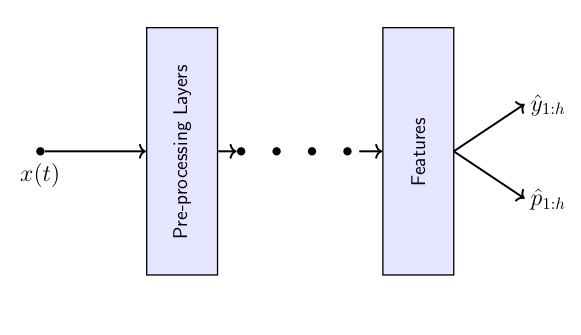
\includegraphics[width=0.5\textwidth]{figures/network.jpg}}
\vspace{.3in}
\caption{Network architecture}
\label{fig:network}
\end{figure}


In section \ref{sec:exp}, we use fully connected neural architectures having a maximum depth of two hidden layers, for prediction of outputs and time lags.

\section{Experiments}\label{sec:exp}


Just as the MNIST, CIFAR Santa Fe Laser and other data sets serve as a way to evaluate machine learning algorithms, it is necessary to propose benchmark problems for \emph{causal dynamic time lag}.

This is particularly challenging given the nature of the CDT problem, although causal time lag
relationships do exist in real world data sets (\cite{doi:10.1002/jgra.50429}, \cite{ZHOU2006195}), it is difficult to find data sets with time lag relationships explicitly annotated.

This barrier can be surpassed in turn by careful construction of synthetic data sets which incorporate dynamic time lag relationships between causes and effects with various complexity.

Synthetic data sets allow us to evaluate the accuracy of both, the output and time lag predictions of CDT models. To this end, we propose four benchmark tests, which are motivated by their connection to the solar wind prediction problem, but which we hope can become canonical examples in the area of CDT modelling.

\subsection{Data Generation}

We start by generating the time series $x(t) \in \mathbb{R}^8$, of size $4000$ (one copy for training and another for test), which represent the driving/causal forces in our system. This can be achieved with good flexibility using \emph{Stochastic Langevin Dynamics} as shown in equation \ref{eq:data}.

\begin{align}
 x(t+1) &= (1 - \tau) x(t) + \mathcal{N}(0, \sigma^2) \label{eq:data}\\
 y(t+\Delta(t)) &= \alpha ||x(t)||^2 \label{eq:outputs}
\end{align}

In equation \ref{eq:outputs} we define the output $y(.)$ as the square norm of the appropriately time lagged input, where $\Delta(t)$ determines the causal time lag relationship.

\subsection{Generating Predictions}

As described in section \ref{sec:model} above, for each input pattern $x(t)$, the model generates two sets of predictions, i.e. ${\hat{y}_i}$, output estimates and probabilities $\hat{p}_i$ for the time window $i \in [t+\ell, t+\ell+h)$ of width $h$. In all of the following benchmarks we set $\ell = 0$ and $h = 20$.

In order to evaluate the model predictions for the benchmarks, we choose the prediction $\hat{y}_j$ which has the highest probability of a causal link $j = {argmax}_{i} \ \hat{p}_i, \forall i \in [t+\ell, t+\ell+h)$. The predictions $(\hat{y}_j, j)$ can now be compared to their corresponding ground truth values $(y(t + \Delta(t)), \Delta(t))$. 

When generating predictions for temporally successive test patters $x'(t)$, it is possible that our model produces time gaps in the reconstruction of the test outputs $y'(t)$. This can happen due to departure from the assumptions outlined in section \ref{sec:formulation}. We can get around these gaps using linear interpolation.


\subsection{Benchmark Problems}\label{sec:benchmark}

Based on the above framework we construct four benchmark problems.

\begin{enumerate}
\item \textbf{Problem I} Constant Lag: \newline 
$\Delta(t) = k$

\item \textbf{Problem II} Constant Velocity $\alpha ||x(t)||^2 + c$; Fixed Distance $d$: 
\newline $\Delta(t) = d/(\alpha ||x(t)||^2 + c),\ \alpha = \frac{100}{8},\ d = 1000,\ c = 40$

\item \textbf{Problem III} Constant Acceleration $a$; Fixed Distance $d$: 
\newline $\Delta(t) = (\sqrt{\alpha^2||x(t)||^4 + 2ad} - \alpha||x(t)||^2)/a,\ \alpha = \frac{50}{8},\ a = 5,\ d = 1000$

\item \textbf{Problem IV} Softplus time lag: 
\newline $\Delta(t) = exp\left(||x(t)||^2\right)/\left(1 + exp(||x(t)||^2)\right)$

\end{enumerate}



\subsection{Results}

The results of the experiments of \ref{sec:benchmark} are evaluated using the following charts.

\begin{enumerate}
    \item Output-Time Lag charts: Since the output time lag relationship can be expressed in closed form, we can visualize this relationship in the generated data sets and evaluate how well the model is able to infer it.
    \item Error Scatter charts: Scatter plots of prediction error in velocity vs prediction error in time lag. They help in visualizing the shape of the error distribution.
\end{enumerate}


\subsubsection{Problem I}

This is the simplest of the benchmark problems, the task is simply to learn a constant time lag from the training data. On the test data set for this problem, the model predicts the correct time lag for $99.92\%$ of the samples. 

With respect to prediction of the outputs, the model has a \emph{mean absolute error} (MAE) of $6.904677$ and achieves a Pearson correlation coefficient of $0.9795$ on a test data set in which the output lies in the range $[9.454, 290.550]$. It should be noted that the $y(t - 1)$ predictor achieves a MAE of $5.186521$ and a Pearson correlation of $0.991$ on this data set. The model is thus able to learn the input-output and time lag mappings easily for this problem.

\begin{figure}[h]
\vspace{.3in}
\centerline{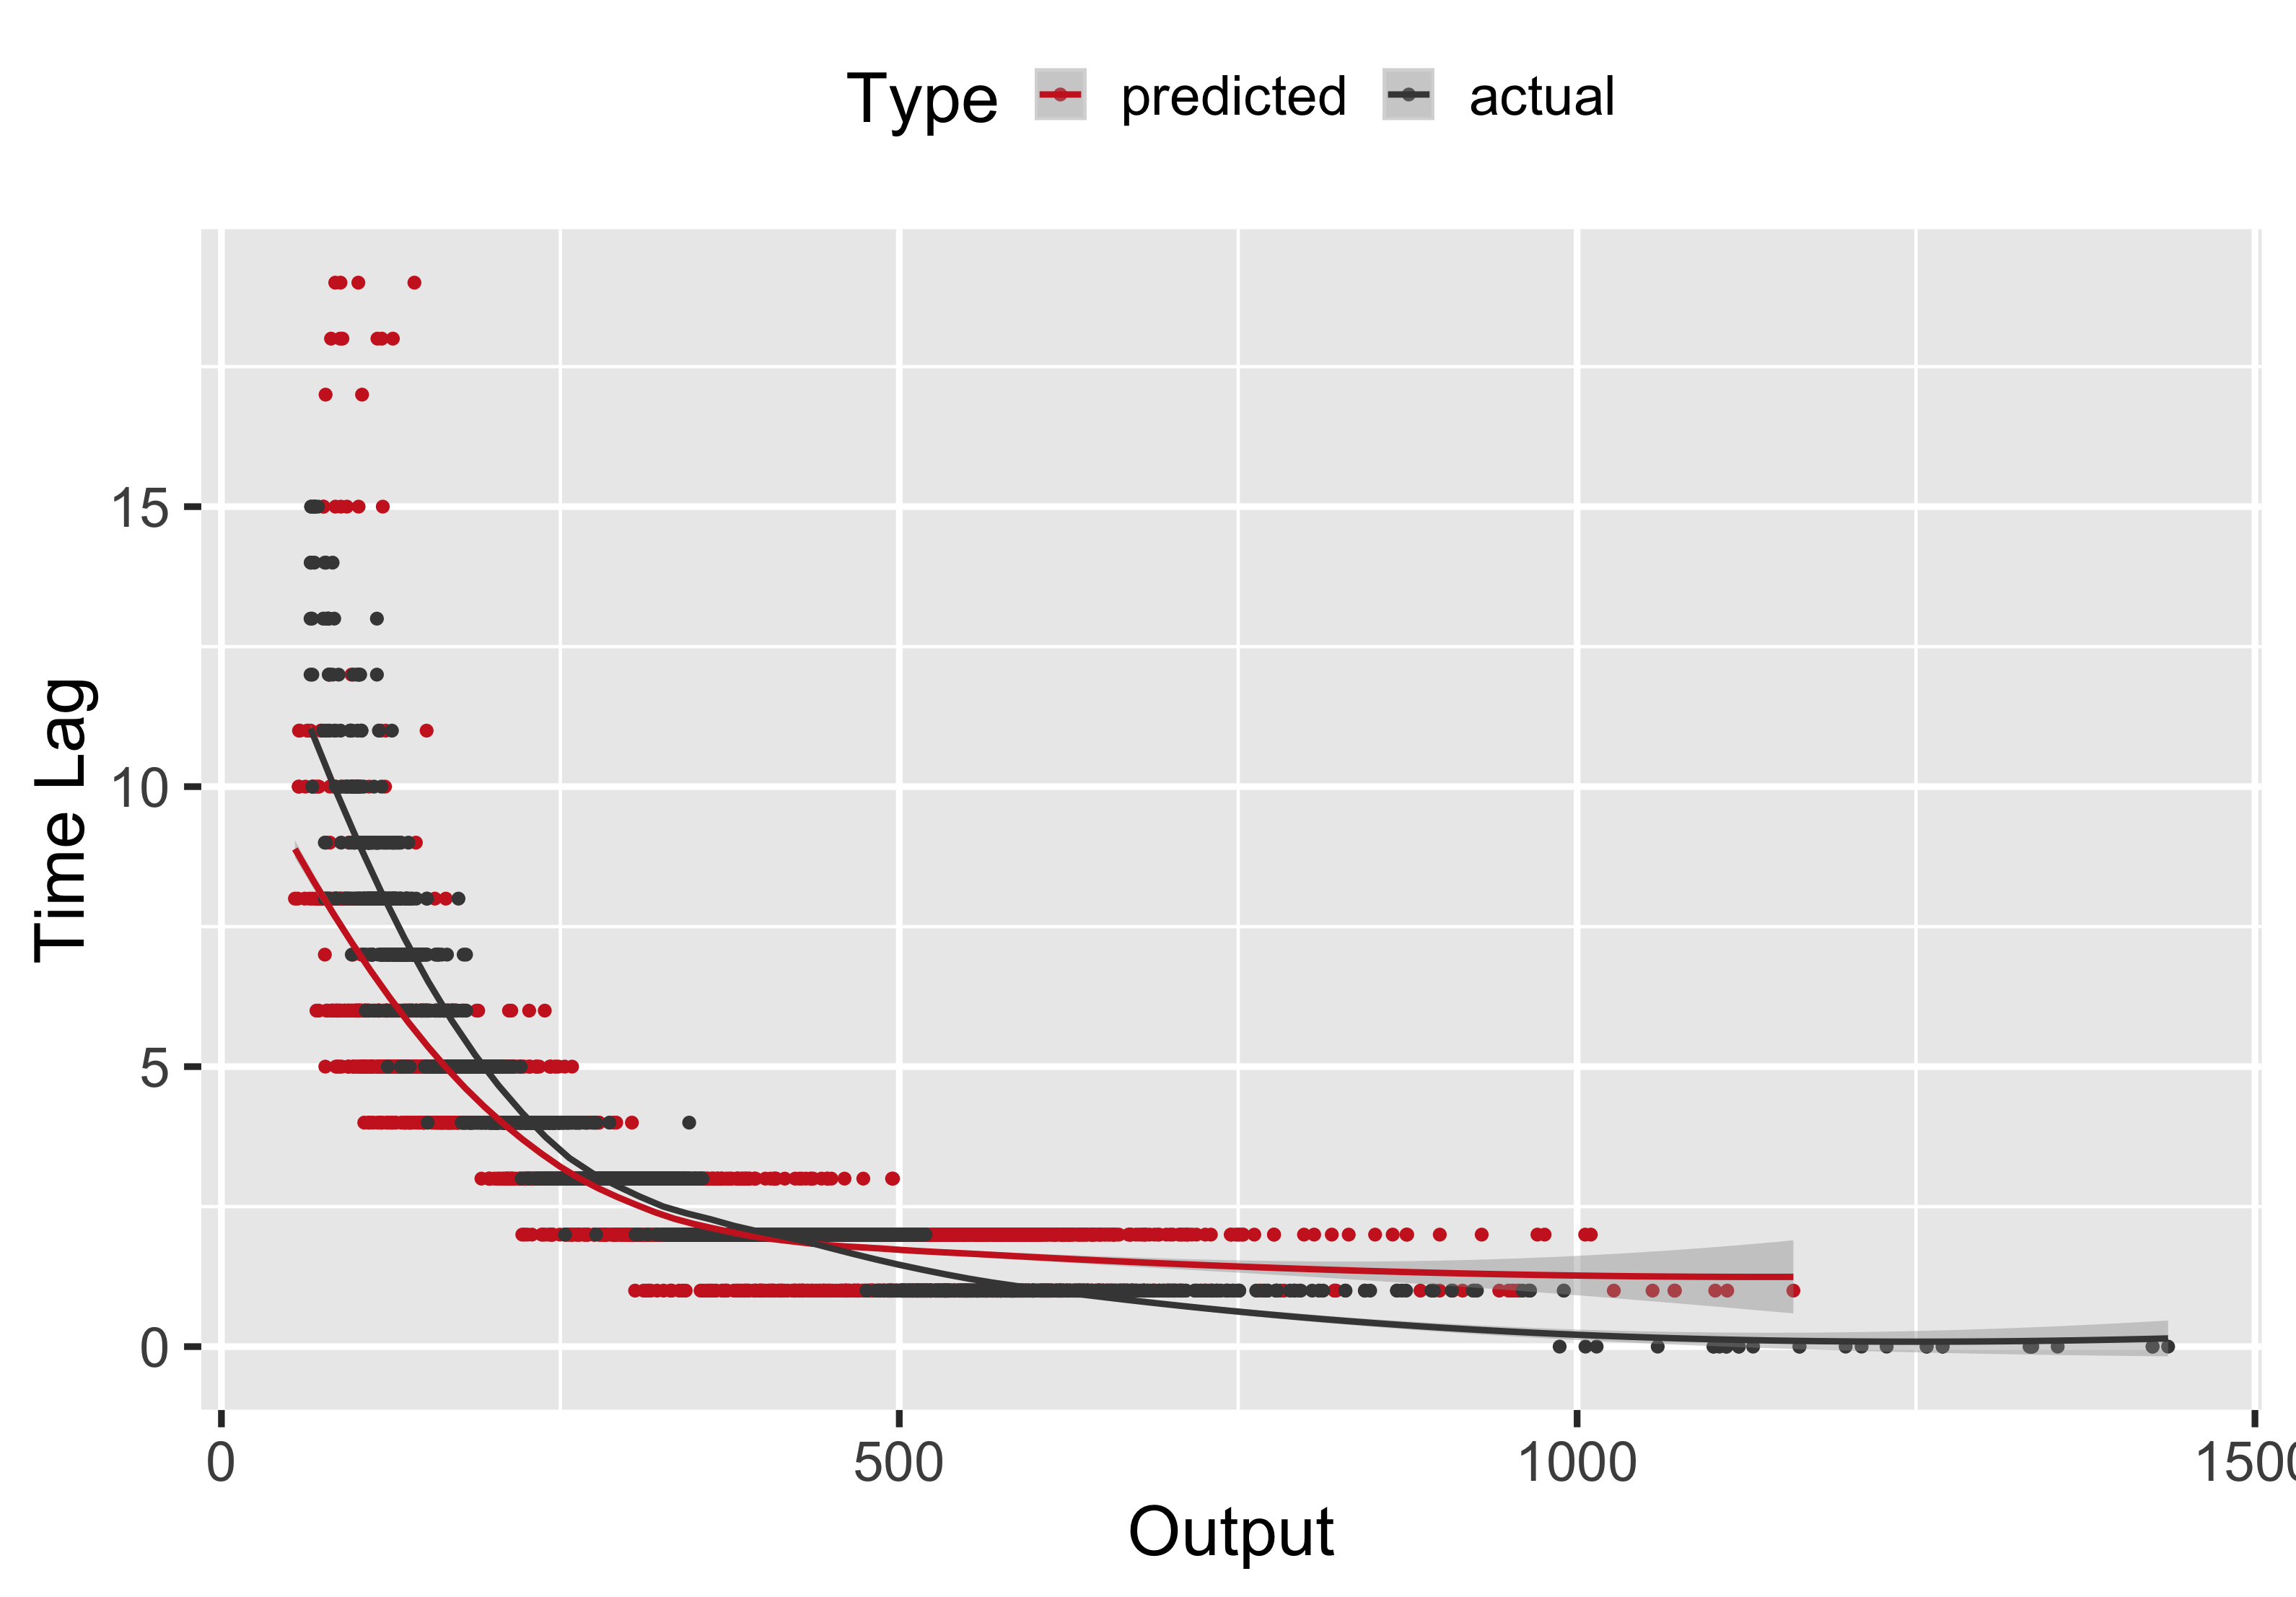
\includegraphics[width=0.5\textwidth]{figures/exp2_scatter_v_tl.png}}
\vspace{.3in}
\caption{\textbf{Problem II}, Output-Time Lag Scatter plot on test data; model predictions in red and actual data in black}
\label{fig:problem2_scatter}
\end{figure}

\begin{figure}[h]
\vspace{.3in}
\centerline{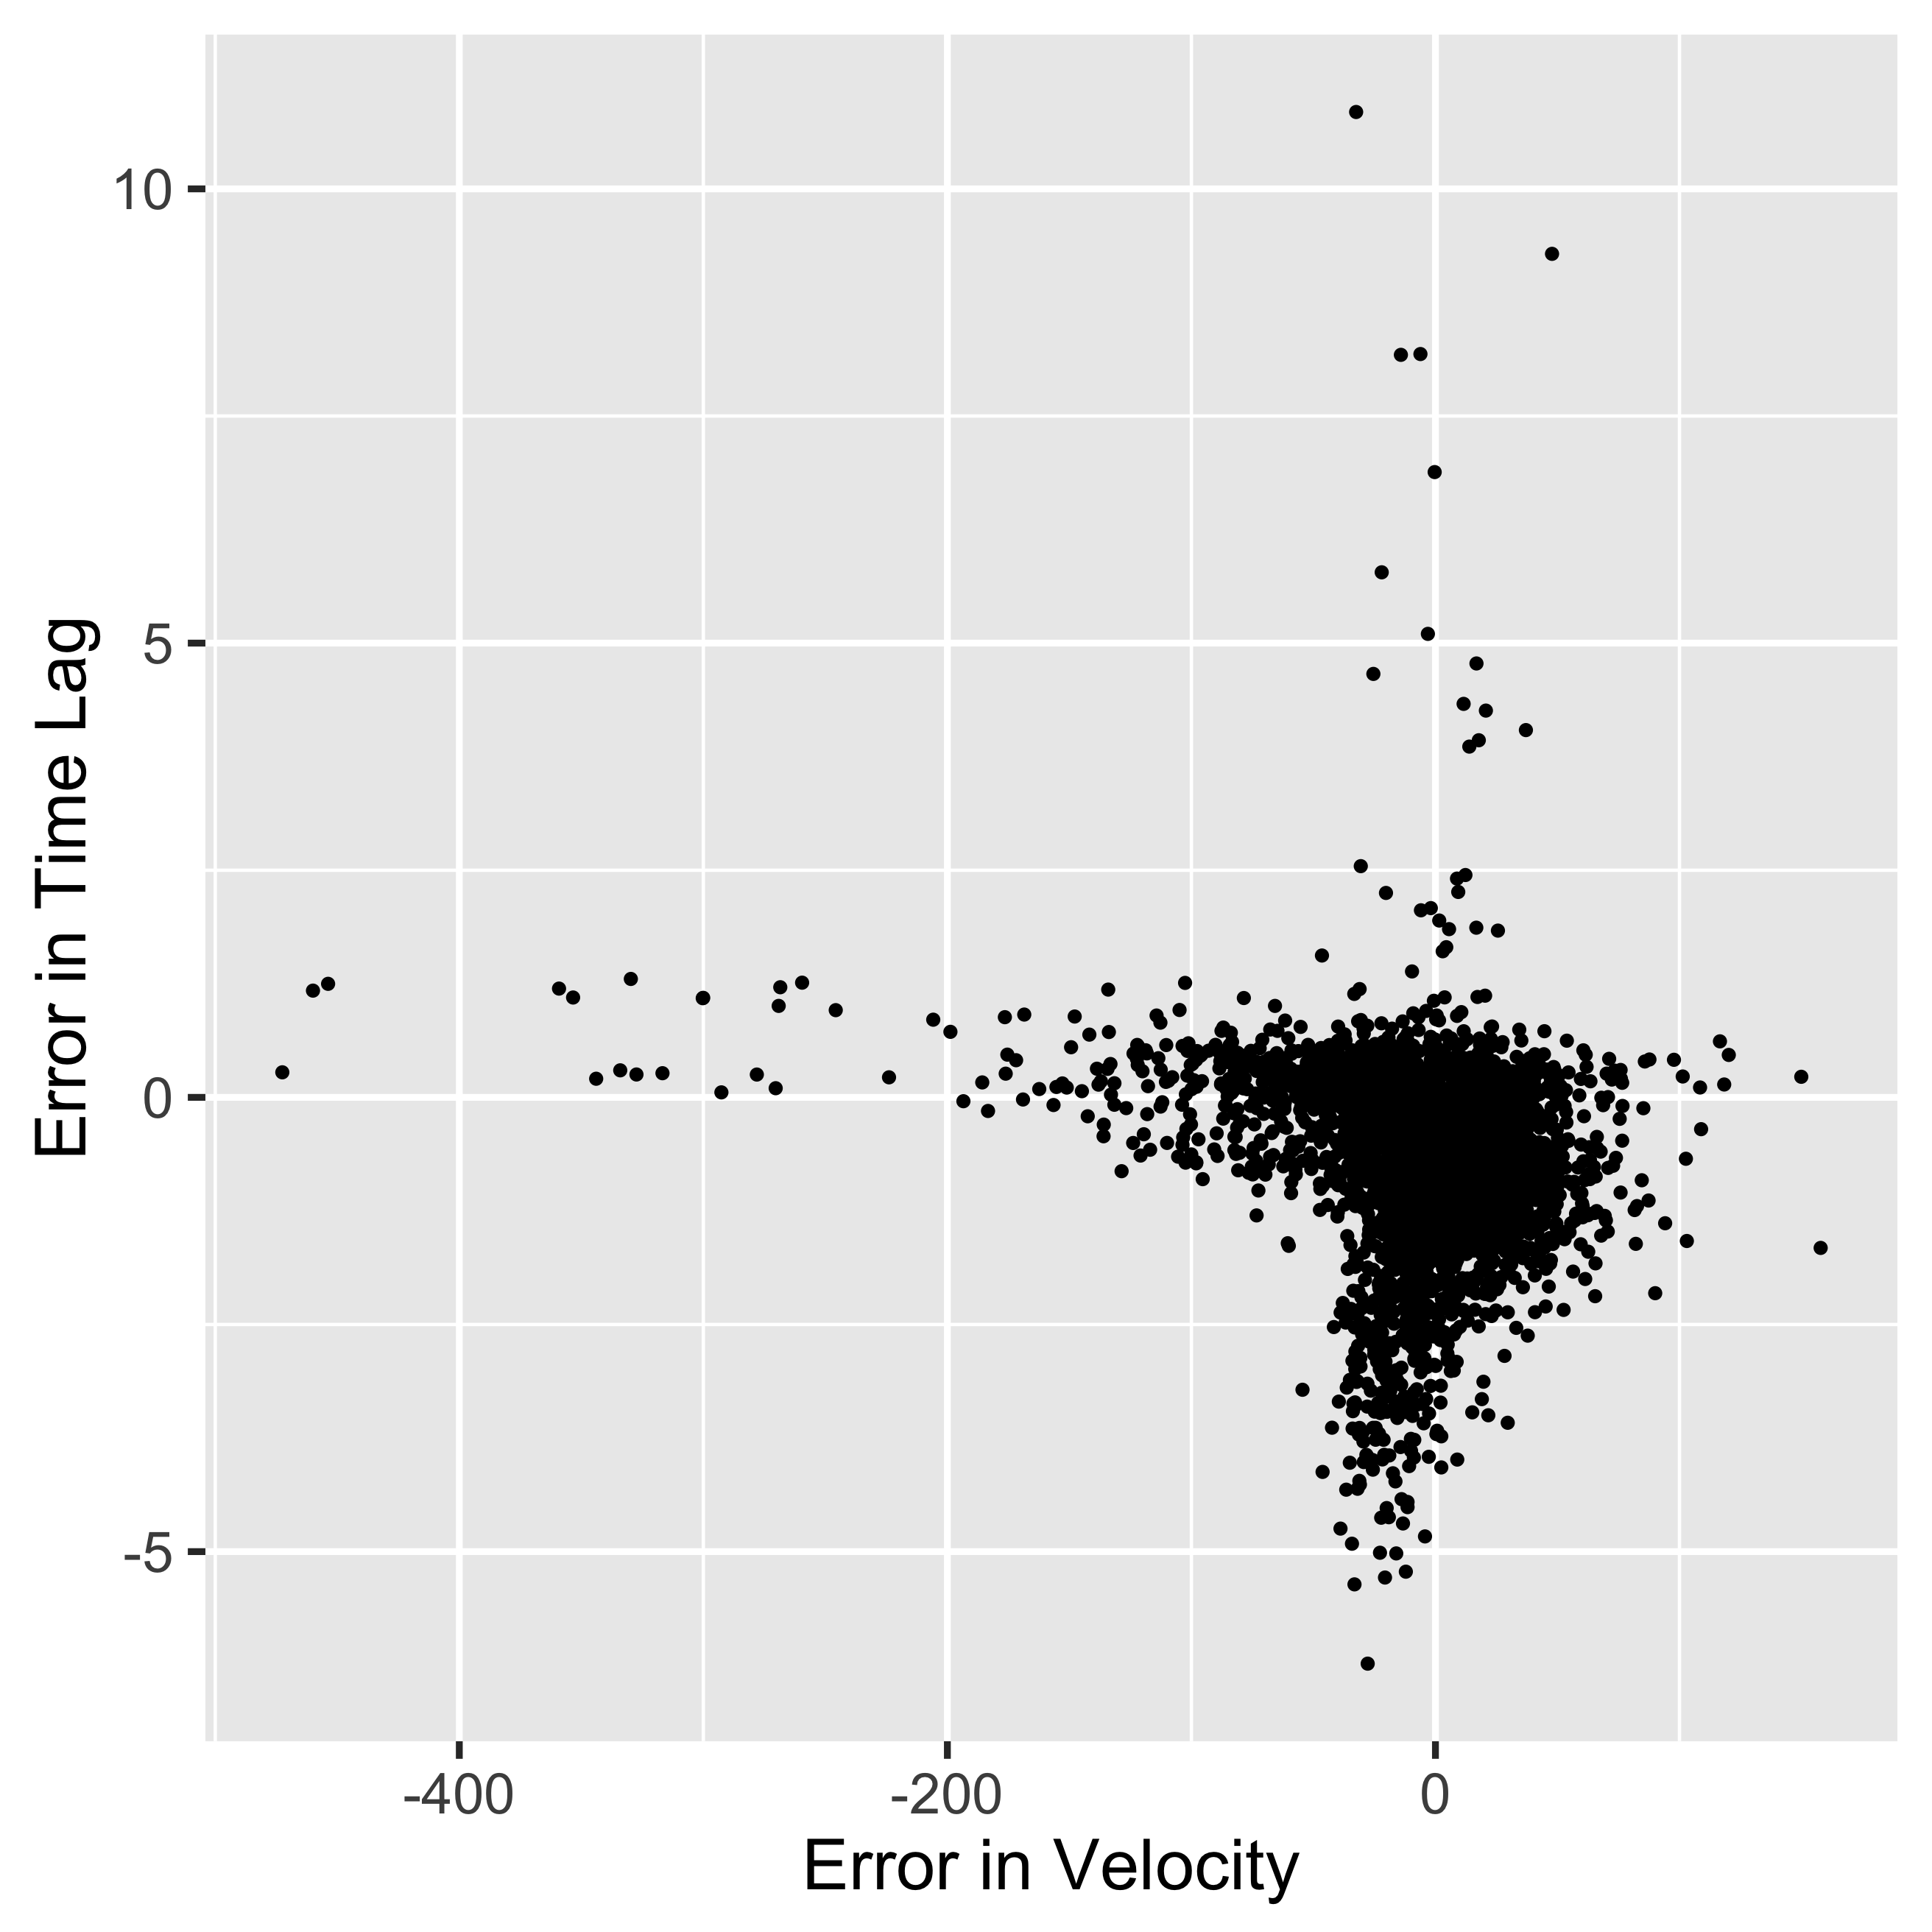
\includegraphics[width=0.5\textwidth]{figures/exp2_scatter_errors_test.png}}
\vspace{.3in}
\caption{\textbf{Problem II}, Error in prediction of output vs error in time lag prediction}
\label{fig:problem2_error}
\end{figure}

\begin{figure}[h]
\vspace{.3in}
\centerline{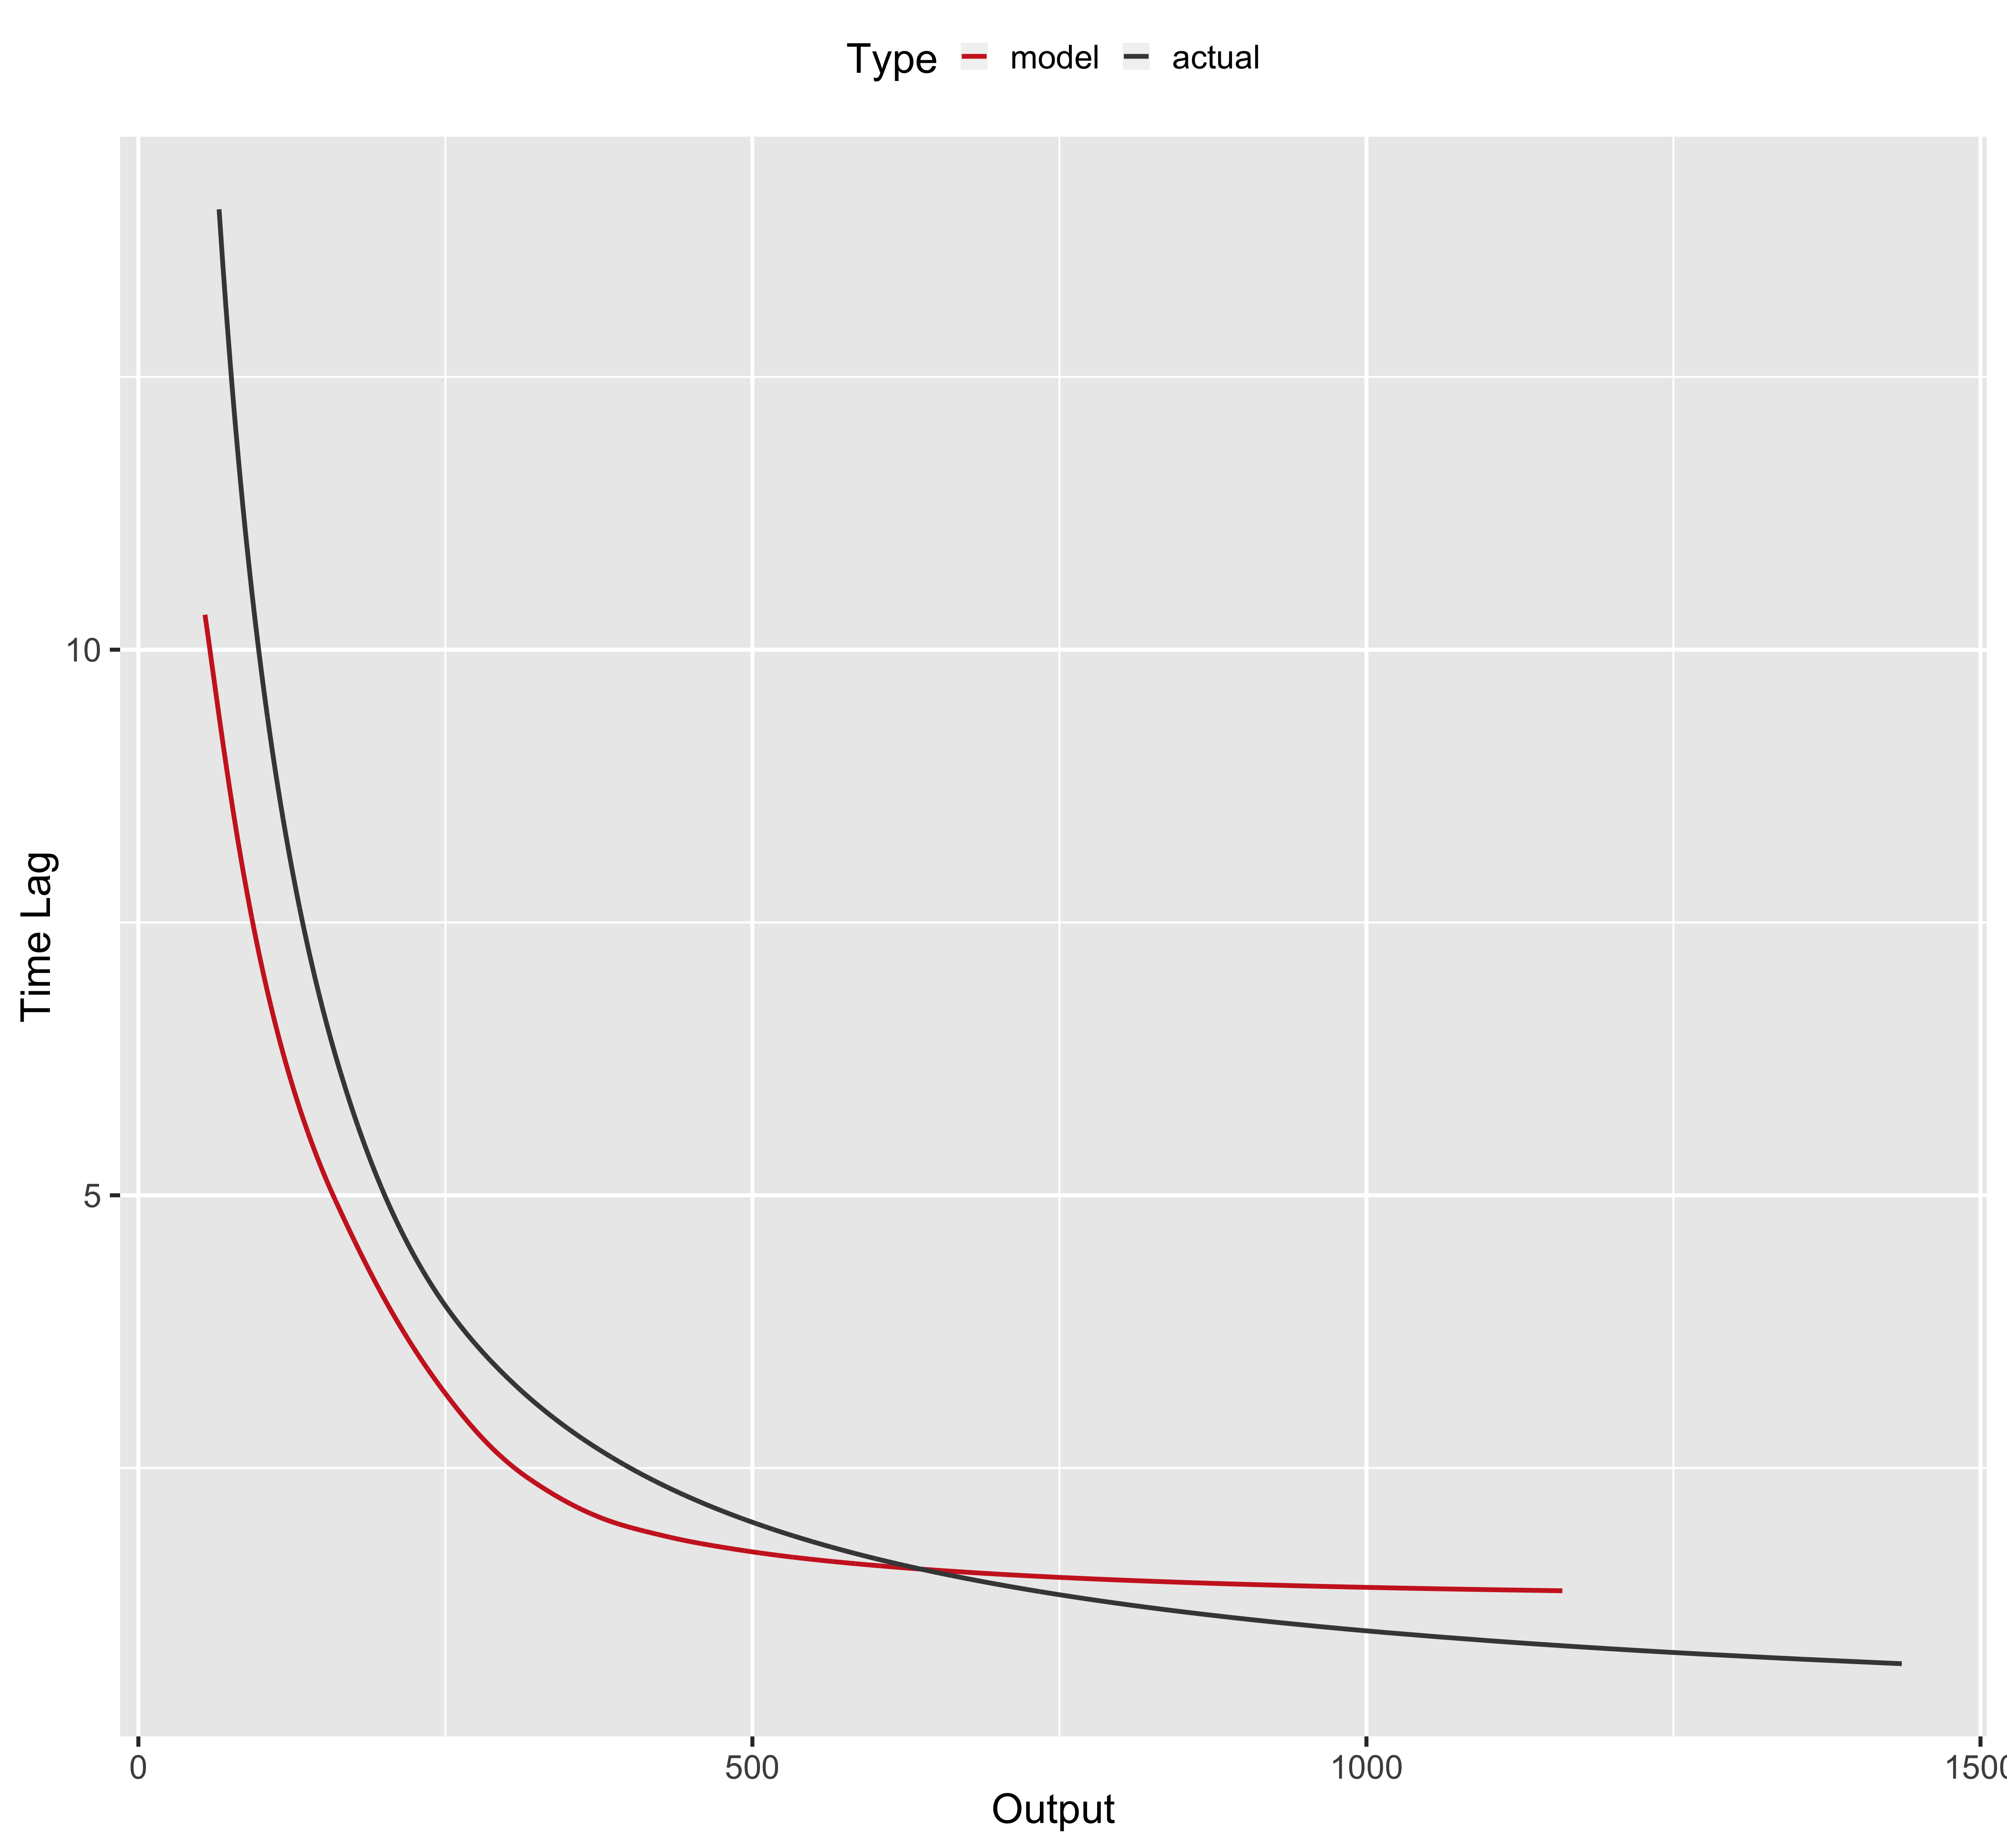
\includegraphics[width=0.5\textwidth]{figures/exp2_predictive_curves.png}}
\vspace{.3in}
\caption{\textbf{Problem II}, Output vs Time Lag Relationship}
\label{fig:problem2_curves}
\end{figure}

\begin{figure}[h]
\vspace{.3in}
\centerline{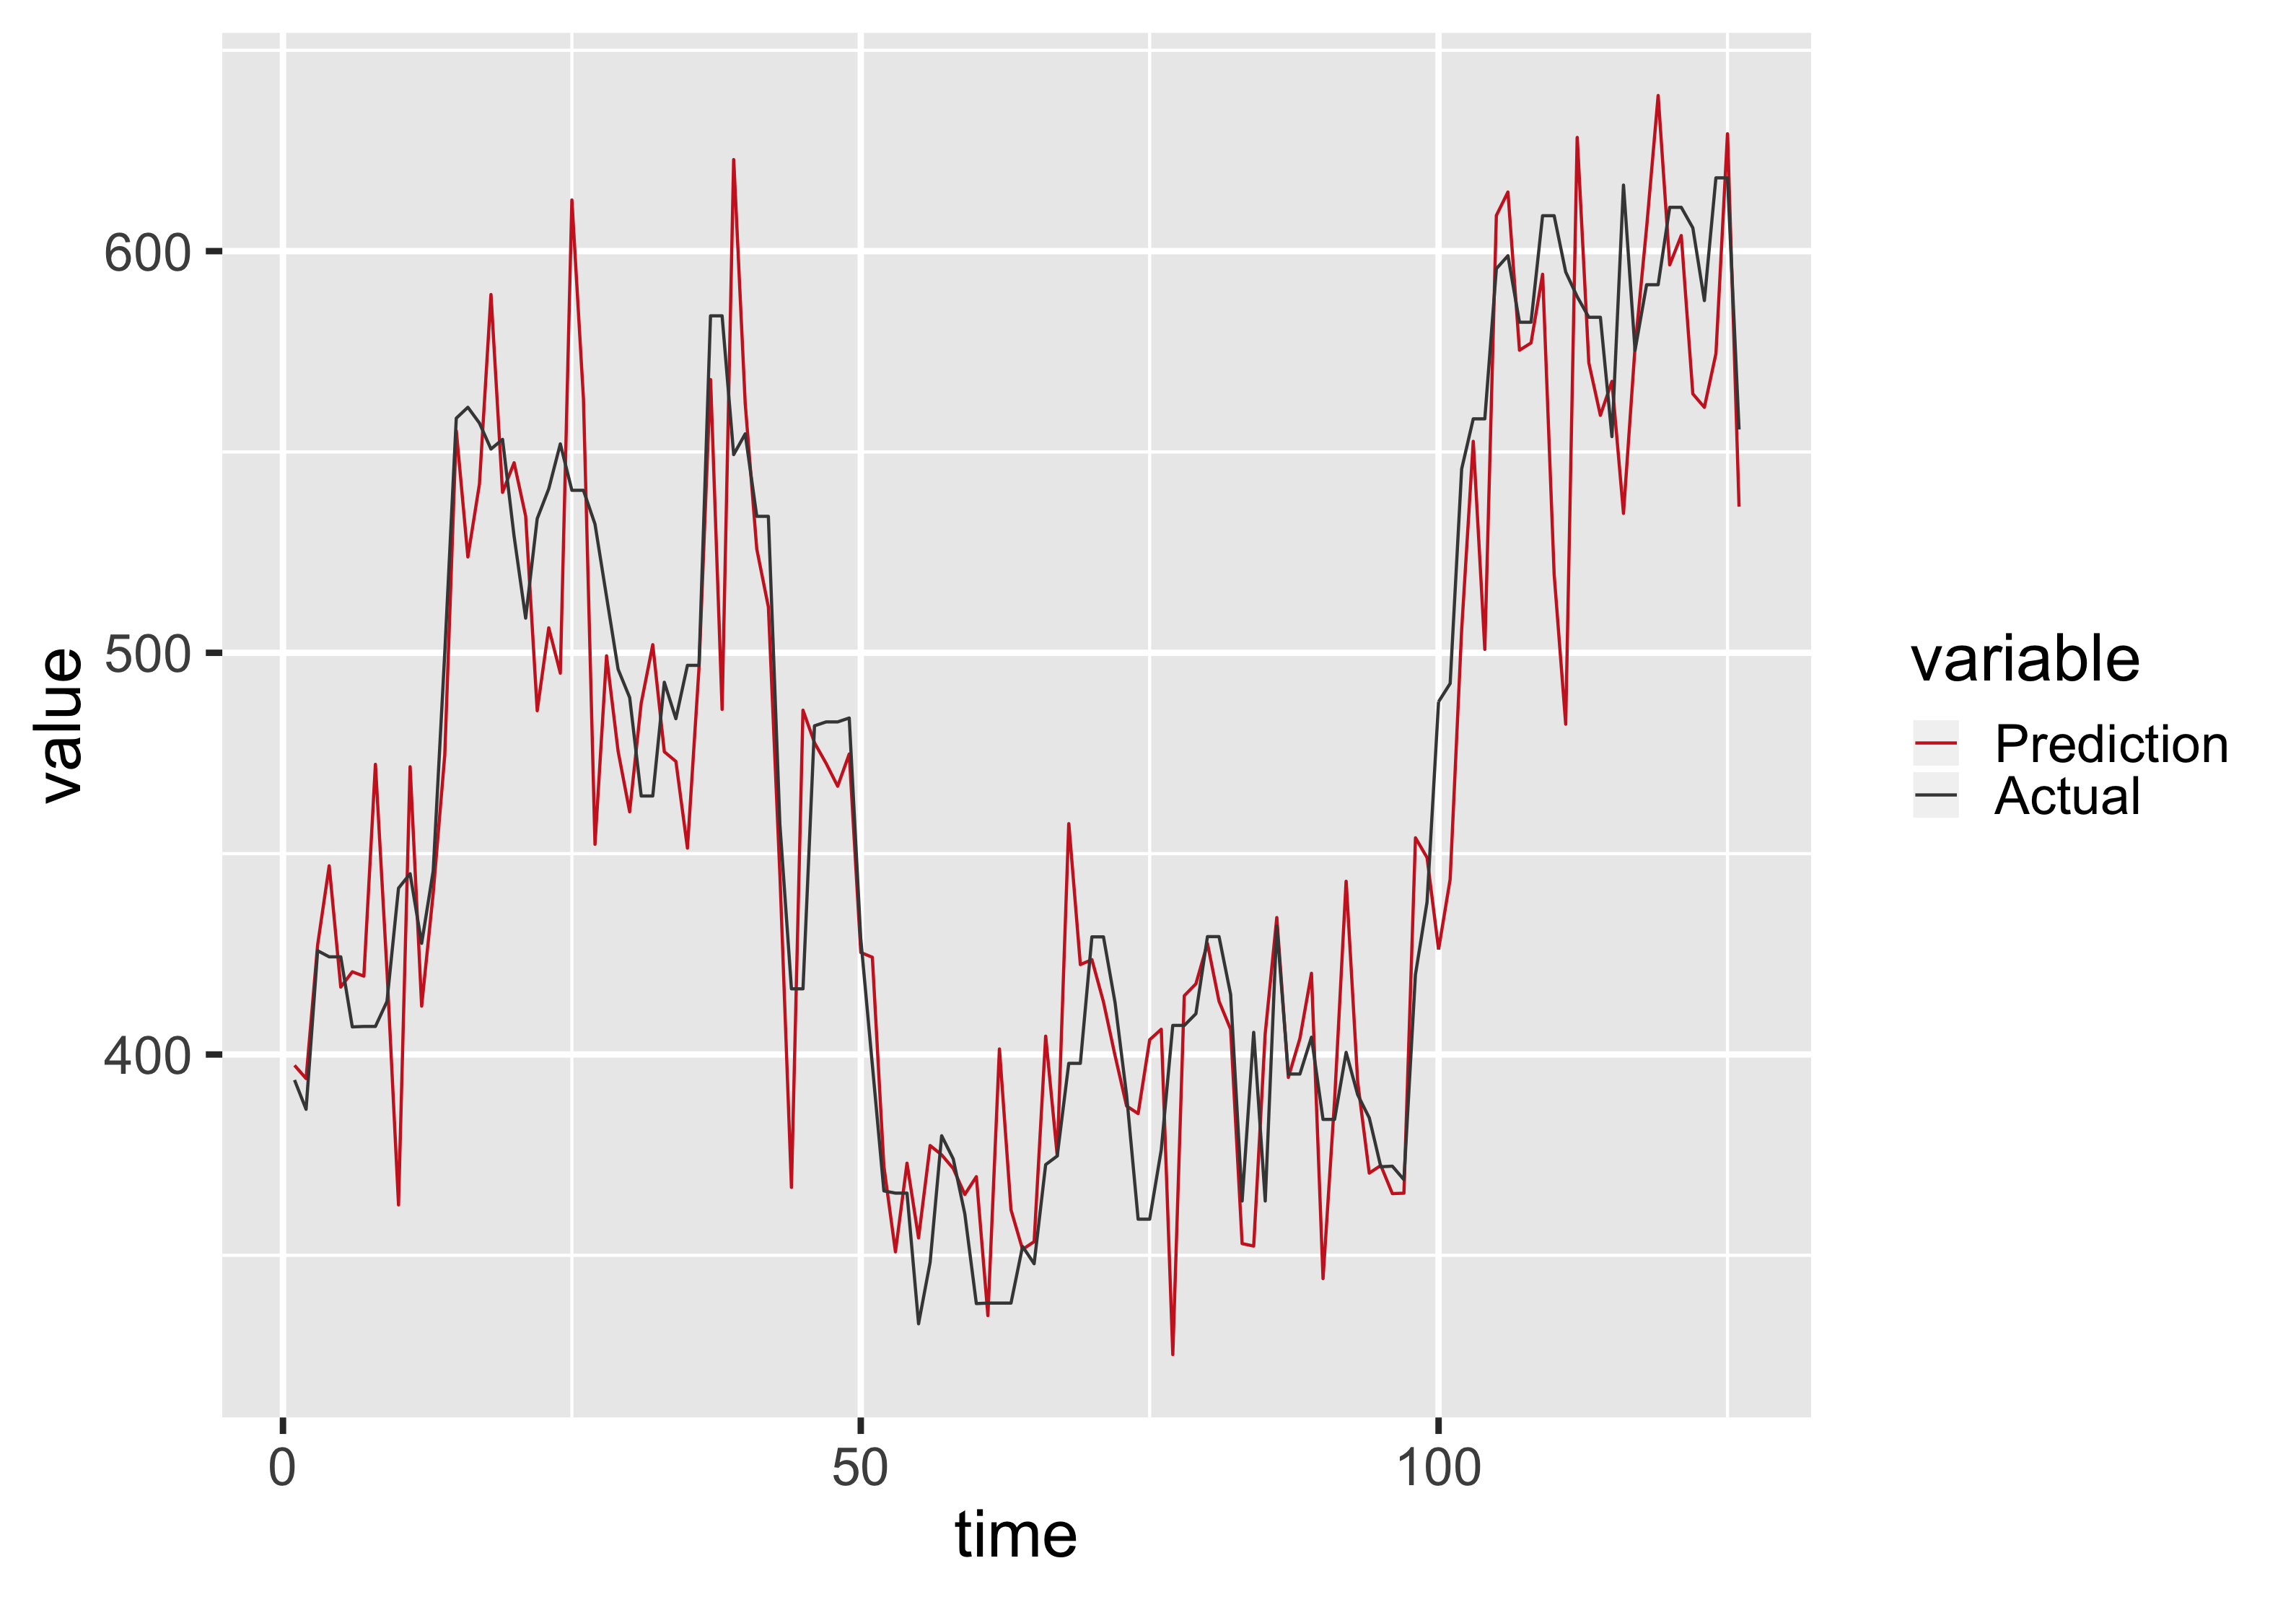
\includegraphics[width=0.5\textwidth]{figures/exp2_timeseries_pred.png}}
\vspace{.3in}
\caption{\textbf{Problem II}, A portion of the test time series reconstructed using the model}
\label{fig:problem2_timeseries}
\end{figure}


\subsubsection{Problem II}

Figure \ref{fig:problem2_scatter} shows a scatter plot between the output value and associated time lag, it compares the scatter distribution generated by the model and compares it with the distribution seen in the test data.

In figure \ref{fig:problem2_error} we present a scatter plot which shows the distribution of the errors in output versus the error in time lag predictions.

In figure \ref{fig:problem2_curves} we present smoothed trends extracted from the data presented in \ref{fig:problem2_scatter}, the red curve represents the output time lag function learned by the model while the black curve is the \emph{ground truth} dependence between the two. 

We can see that the model is able to approximate the inverse relationship between the output and time lag from the training data.

\begin{figure}[h]
\vspace{.3in}
\centerline{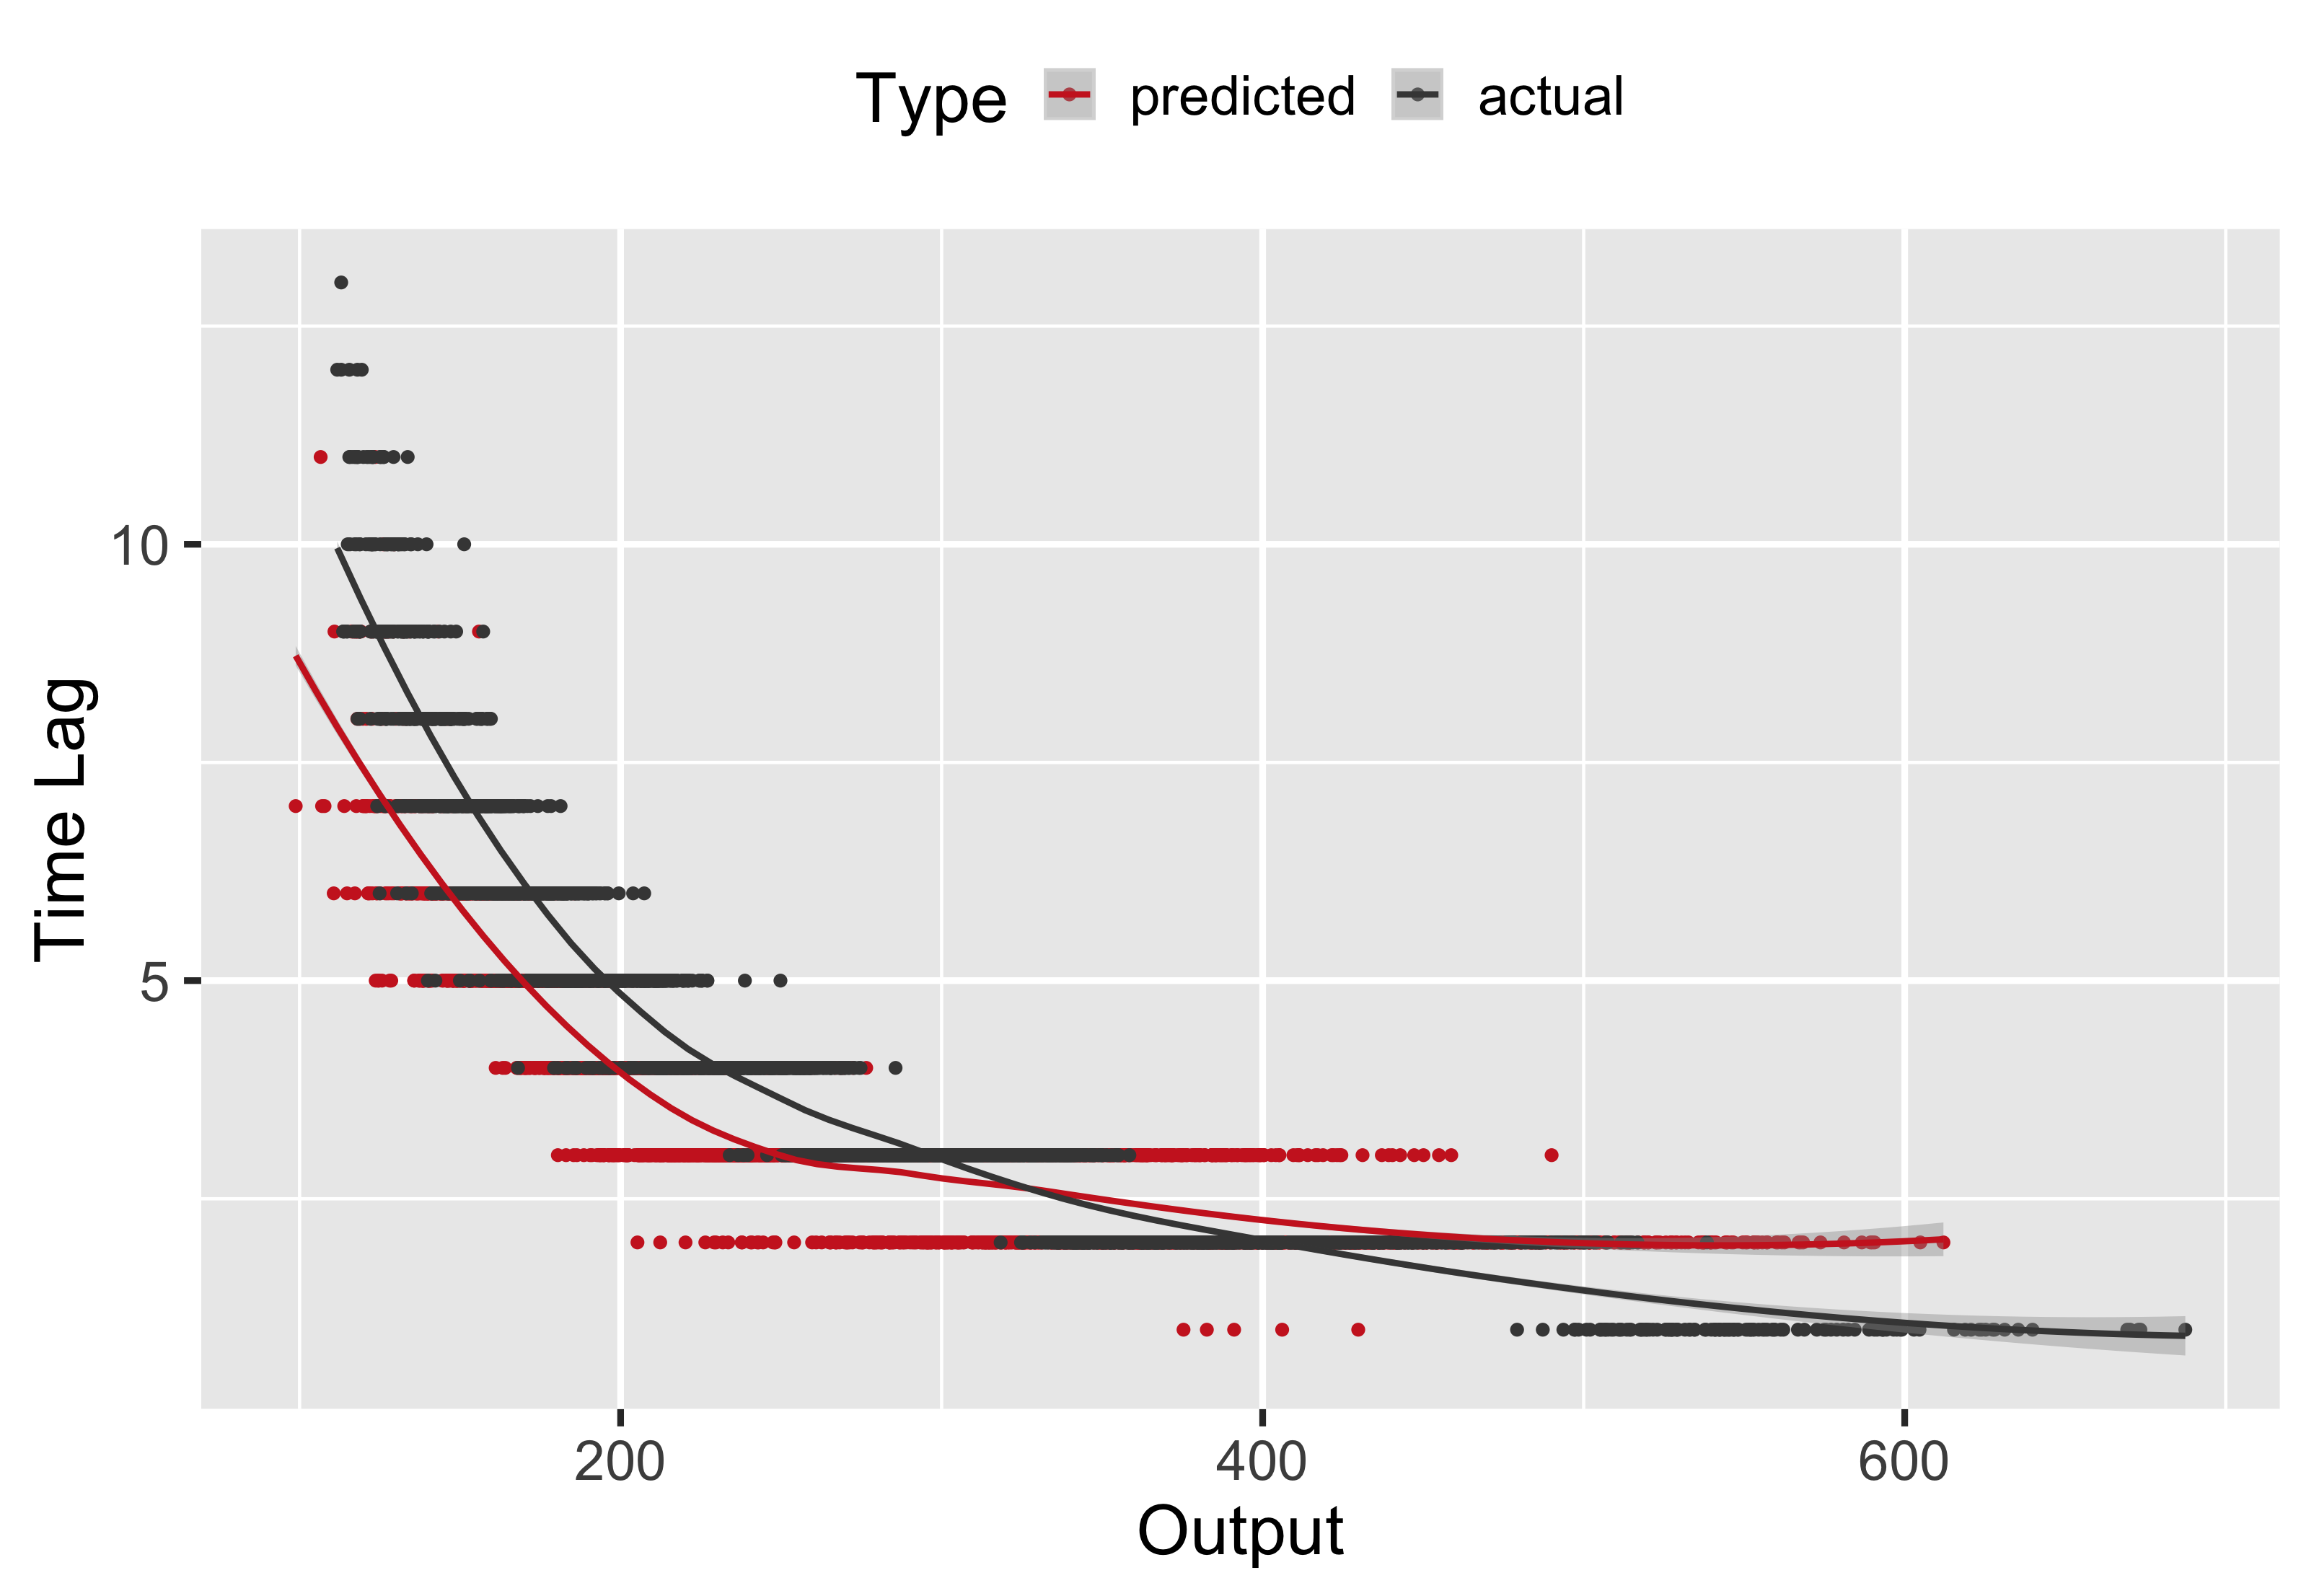
\includegraphics[width=0.5\textwidth]{figures/exp3_scatter_v_tl.png}}
\vspace{.3in}
\caption{\textbf{Problem III}, Output-Time Lag Scatter plot; model predictions in red and actual data in black}
\label{fig:problem3_scatter}
\end{figure}

\begin{figure}[h]
\vspace{.3in}
\centerline{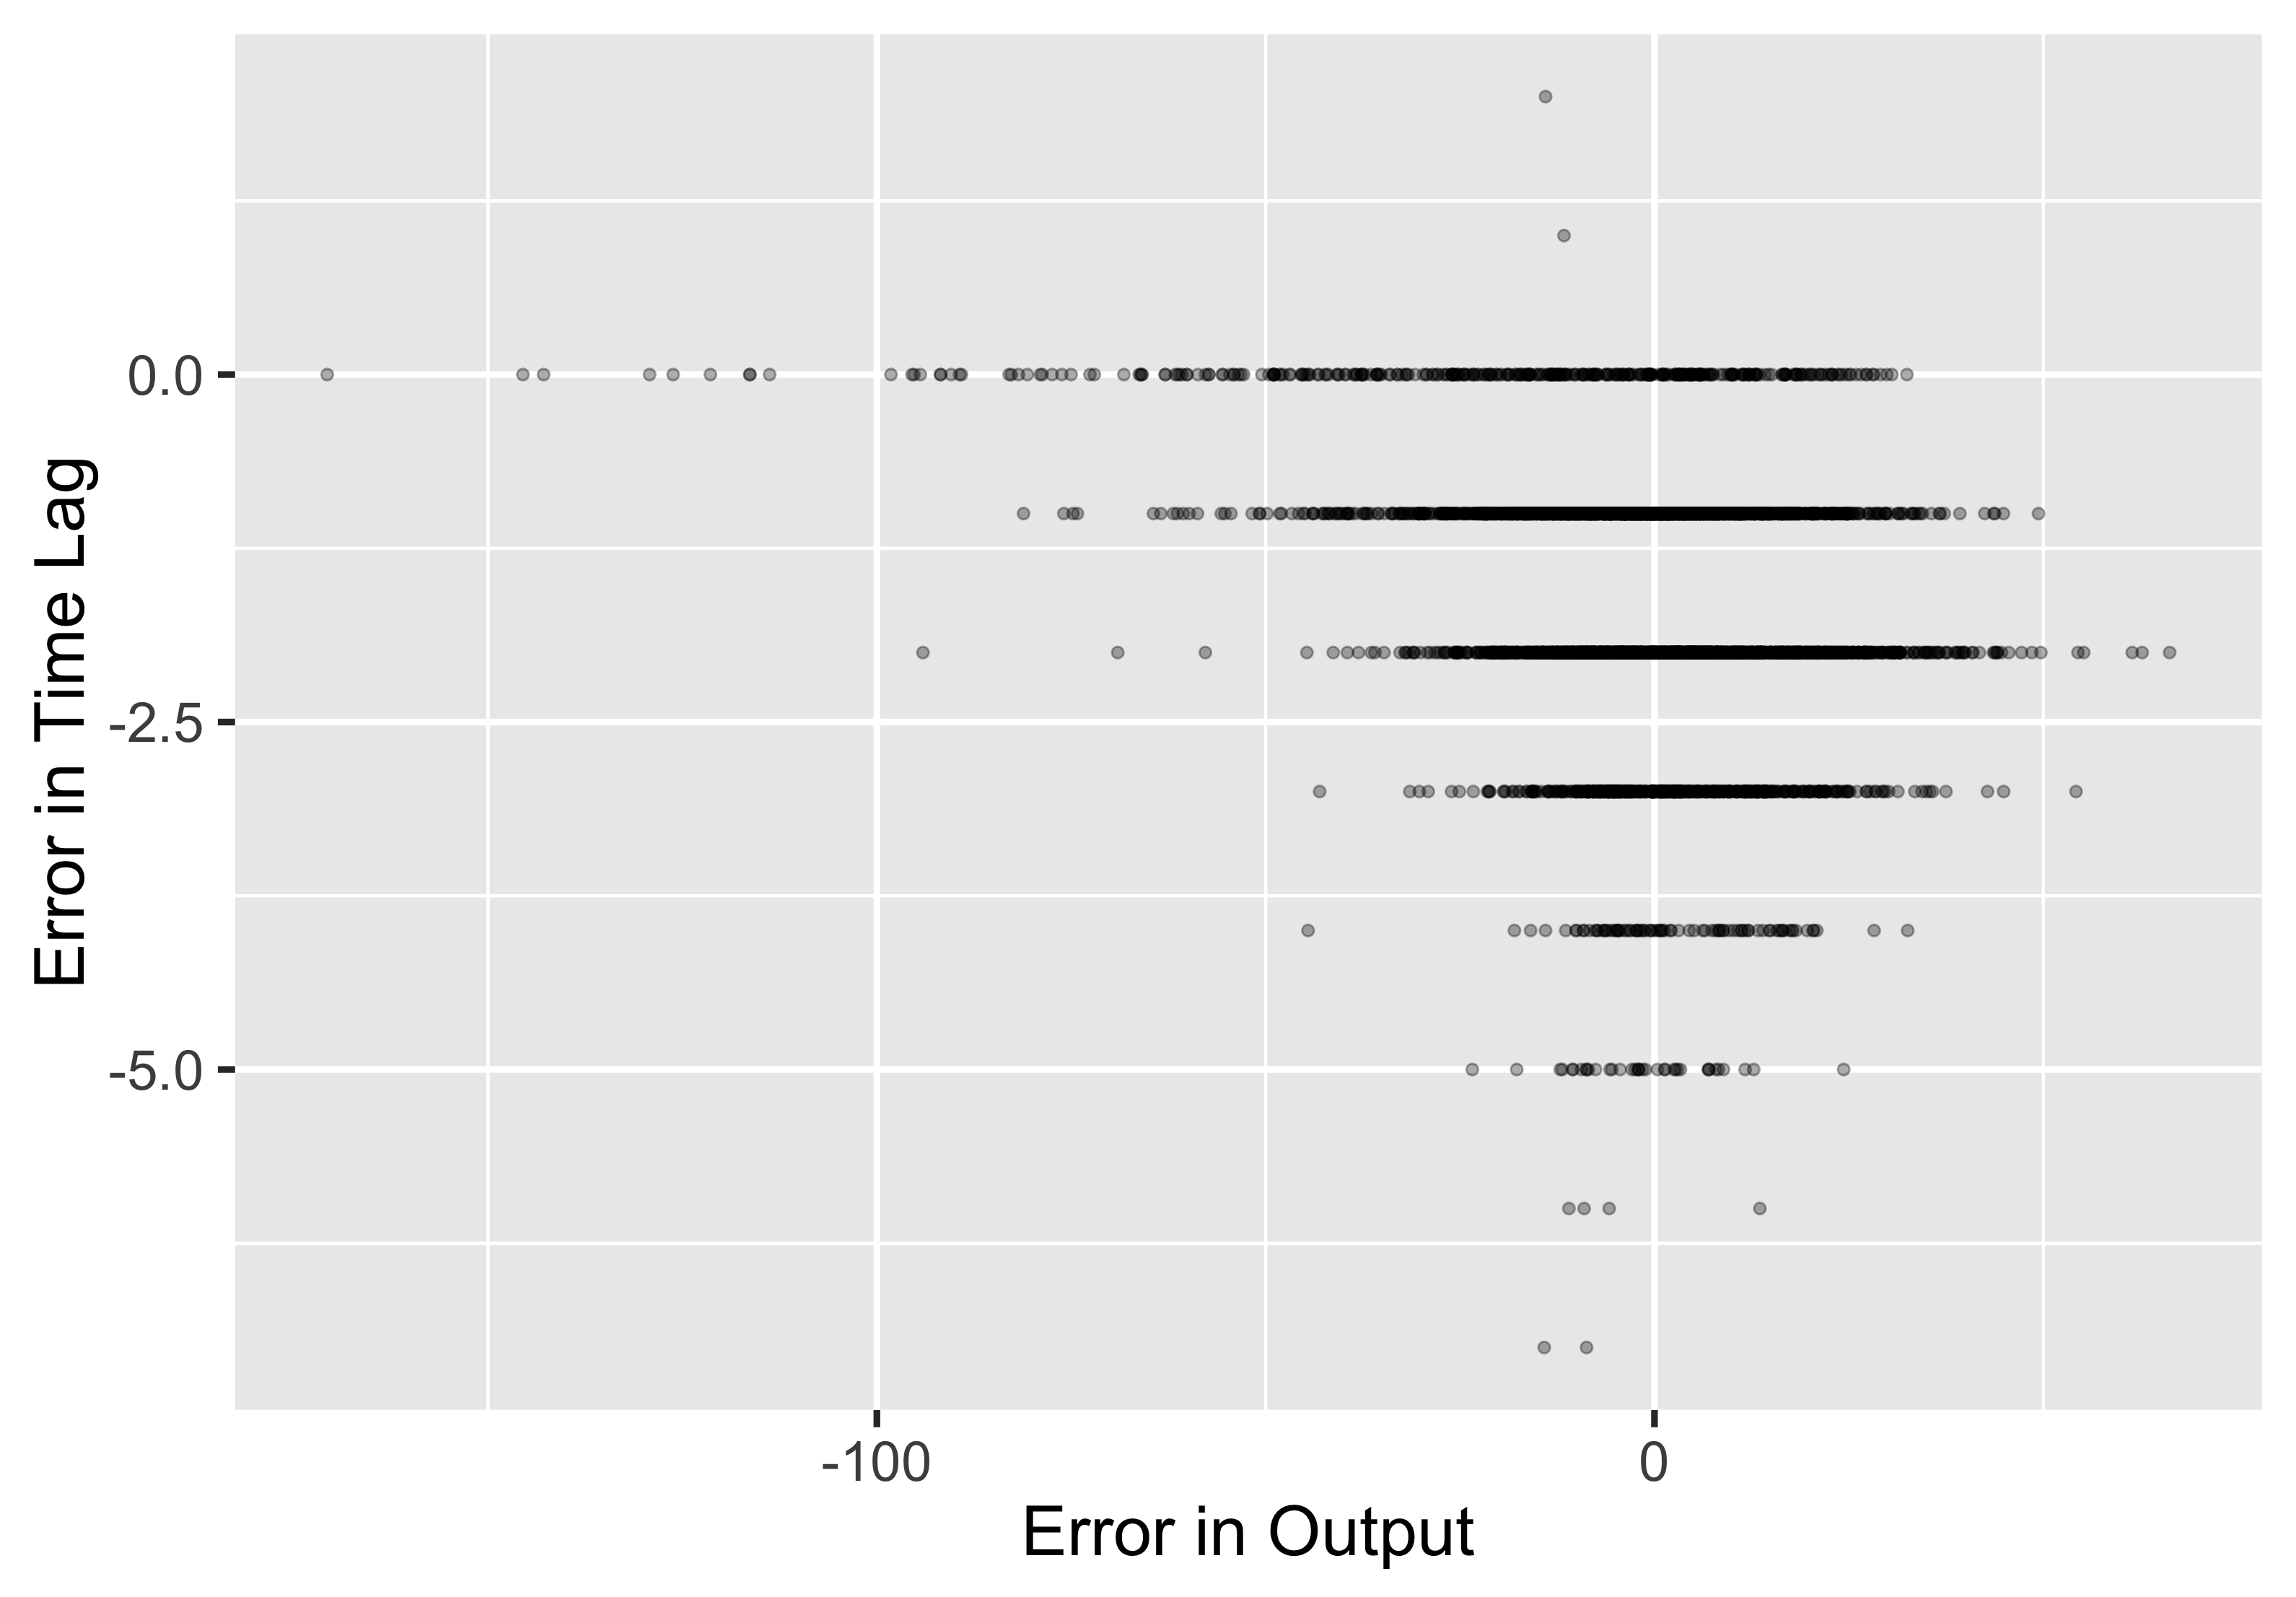
\includegraphics[width=0.5\textwidth]{figures/exp3_scatter_errors_test.png}}
\vspace{.3in}
\caption{\textbf{Problem III}, Error in prediction of output vs error in time lag prediction}
\label{fig:problem3_error}
\end{figure}

\begin{figure}[h]
\vspace{.3in}
\centerline{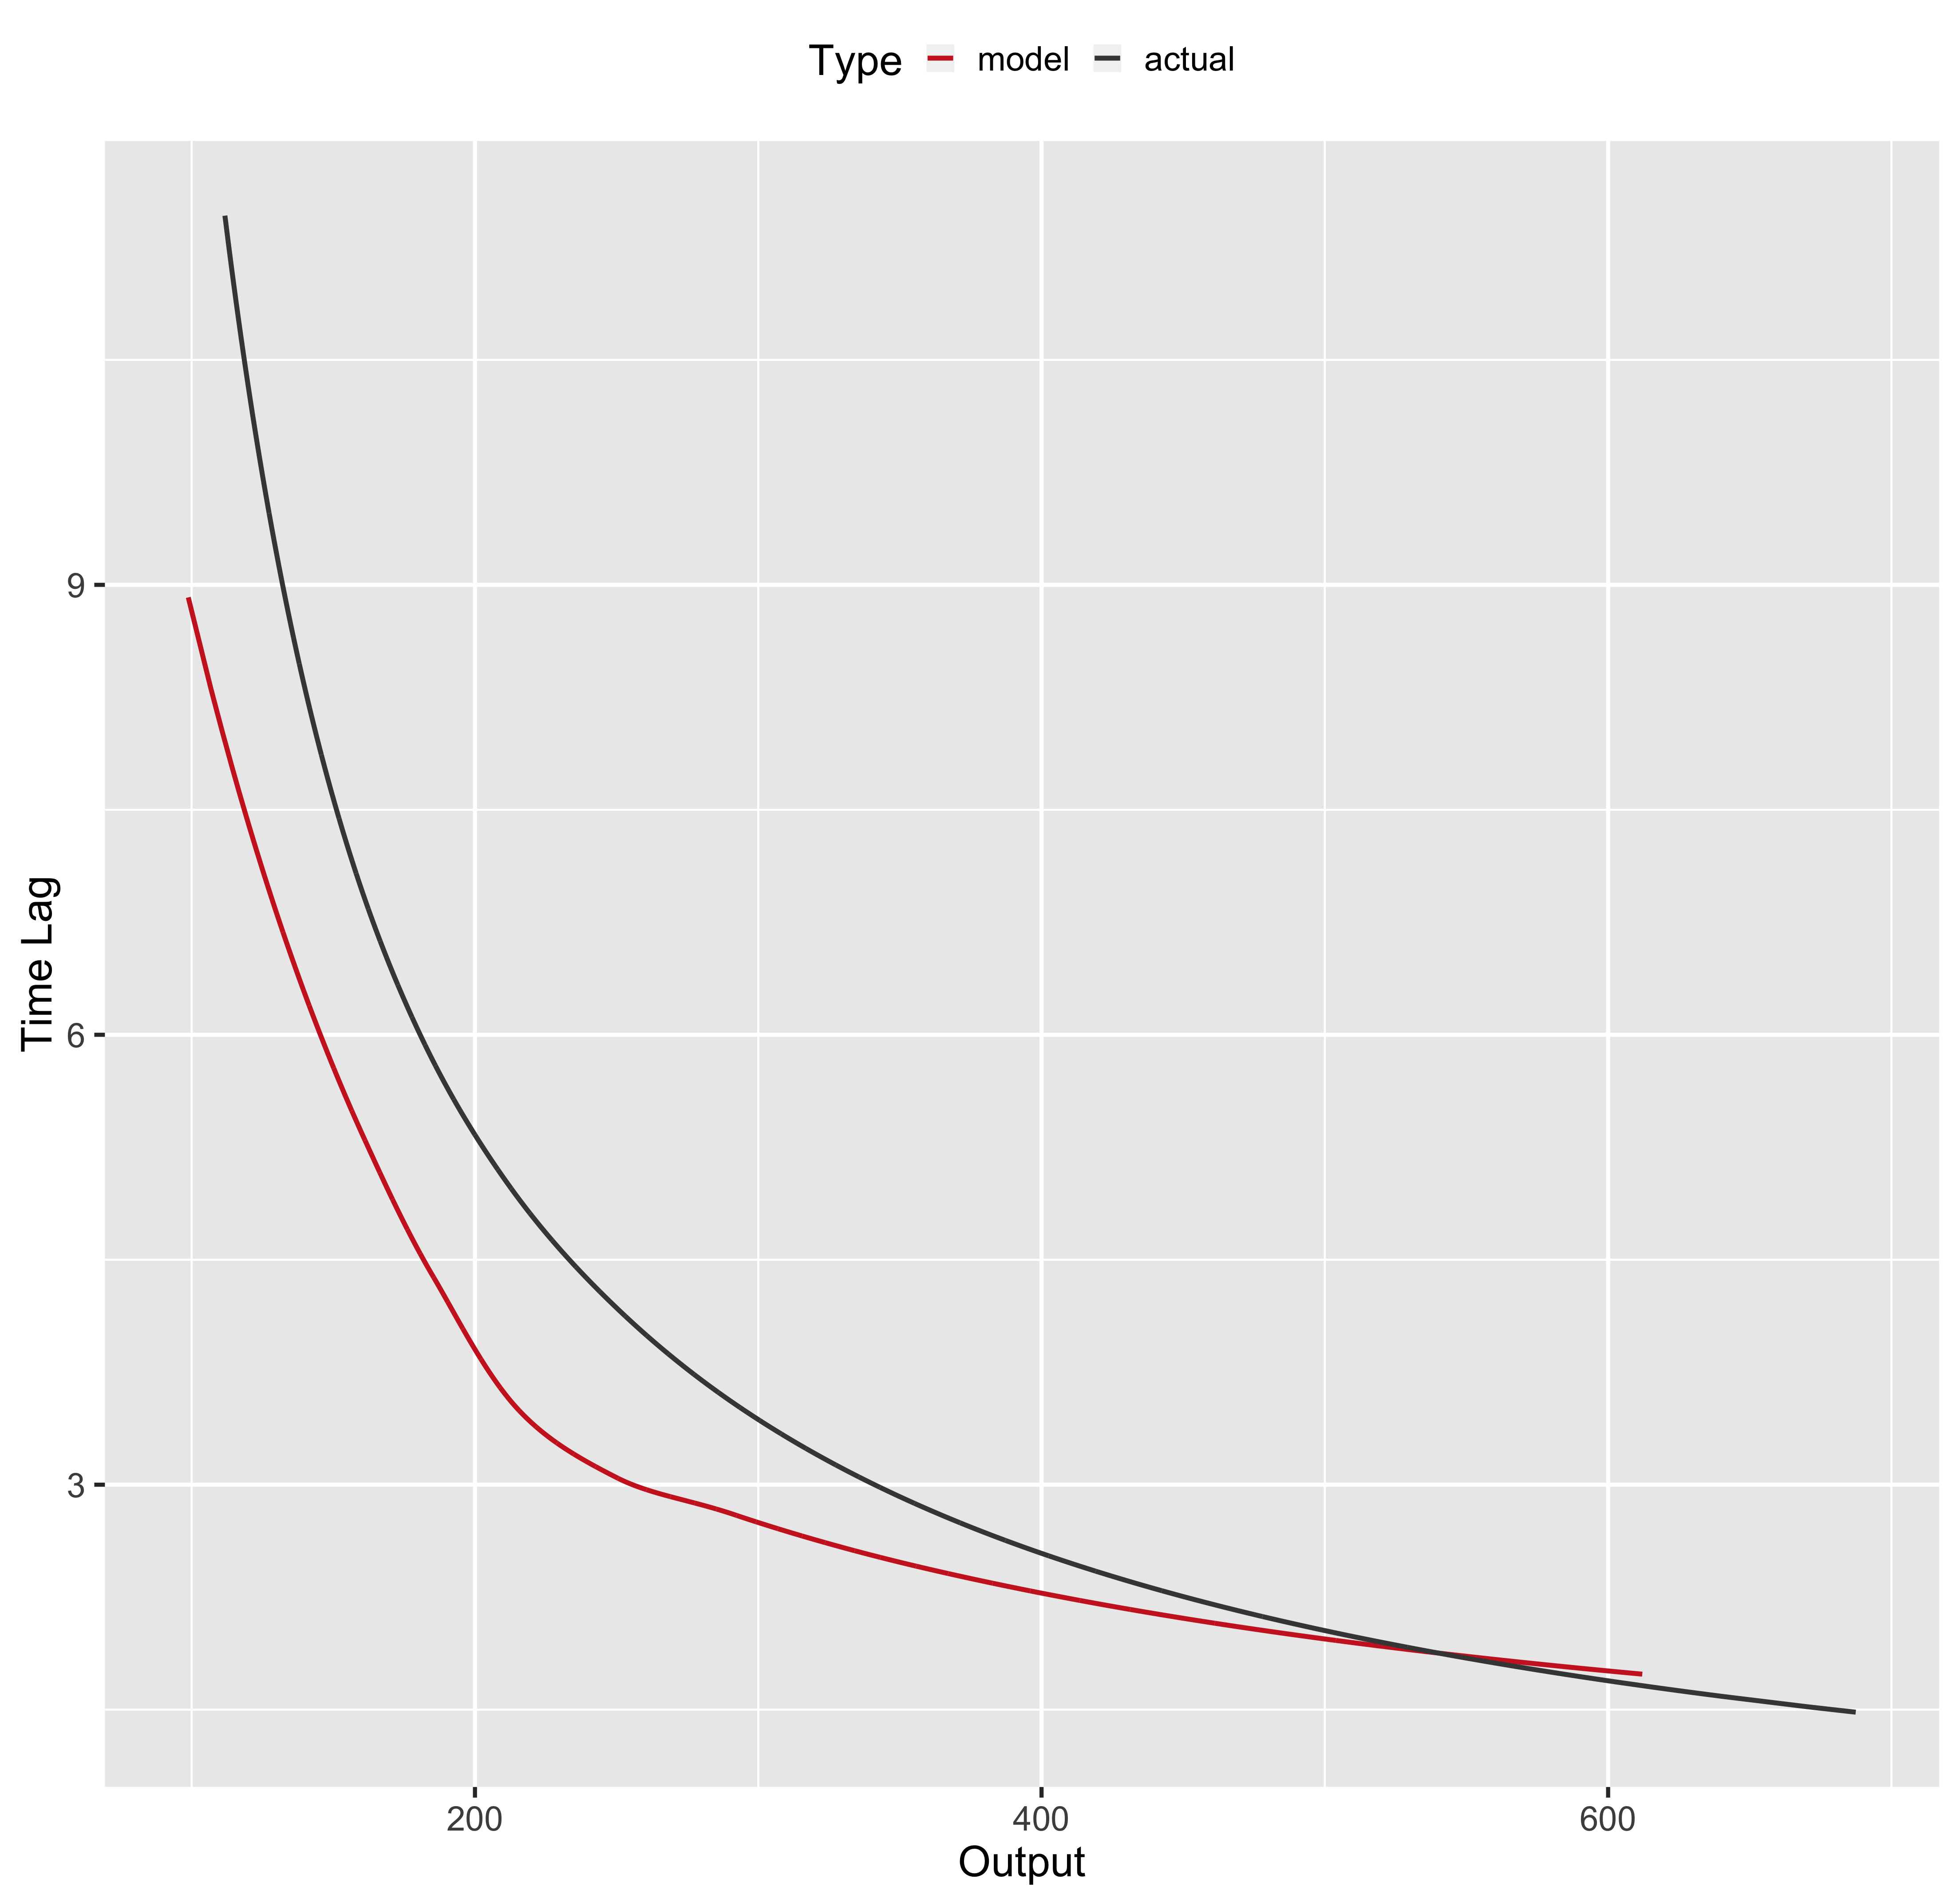
\includegraphics[width=0.5\textwidth]{figures/exp3_predictive_curves.png}}
\vspace{.3in}
\caption{\textbf{Problem III}, Output vs Time Lag Relationship}
\label{fig:problem3_curves}
\end{figure}


\subsubsection{Problem III}

Problem III involves a more complicated output time lag relationship than problem II due to the effect of acceleration. From figures \ref{fig:problem3_scatter} and \ref{fig:problem3_error}, it can be observed that the model can still learn the time lag and output mappings although in this case the time lag error distribution has a slightly longer tail in figure \ref{fig:problem3_error} as compared to \ref{fig:problem2_error}.

One observation common to the results of problems II and III is that the error distribution of the time lag is asymmetric, the model tends to underestimate the time lag. Upon closer examination of the predictions (figure \ref{fig:problem3_lag_error_jus}), it is observed that the data patterns for which the model has a time lag prediction error $\leq -2.5$, tend to occur in lower region of the output space (table \ref{table:problem3_stats}).

It is thus the case that for applications where there is an inverse relationship between the output and time lag, the model's time lag errors are expected to be biased towards the negative region, but when output and time lag are positively correlated, the time lag errors should be unbiased.

\begin{figure}[h]
\vspace{.3in}
\centerline{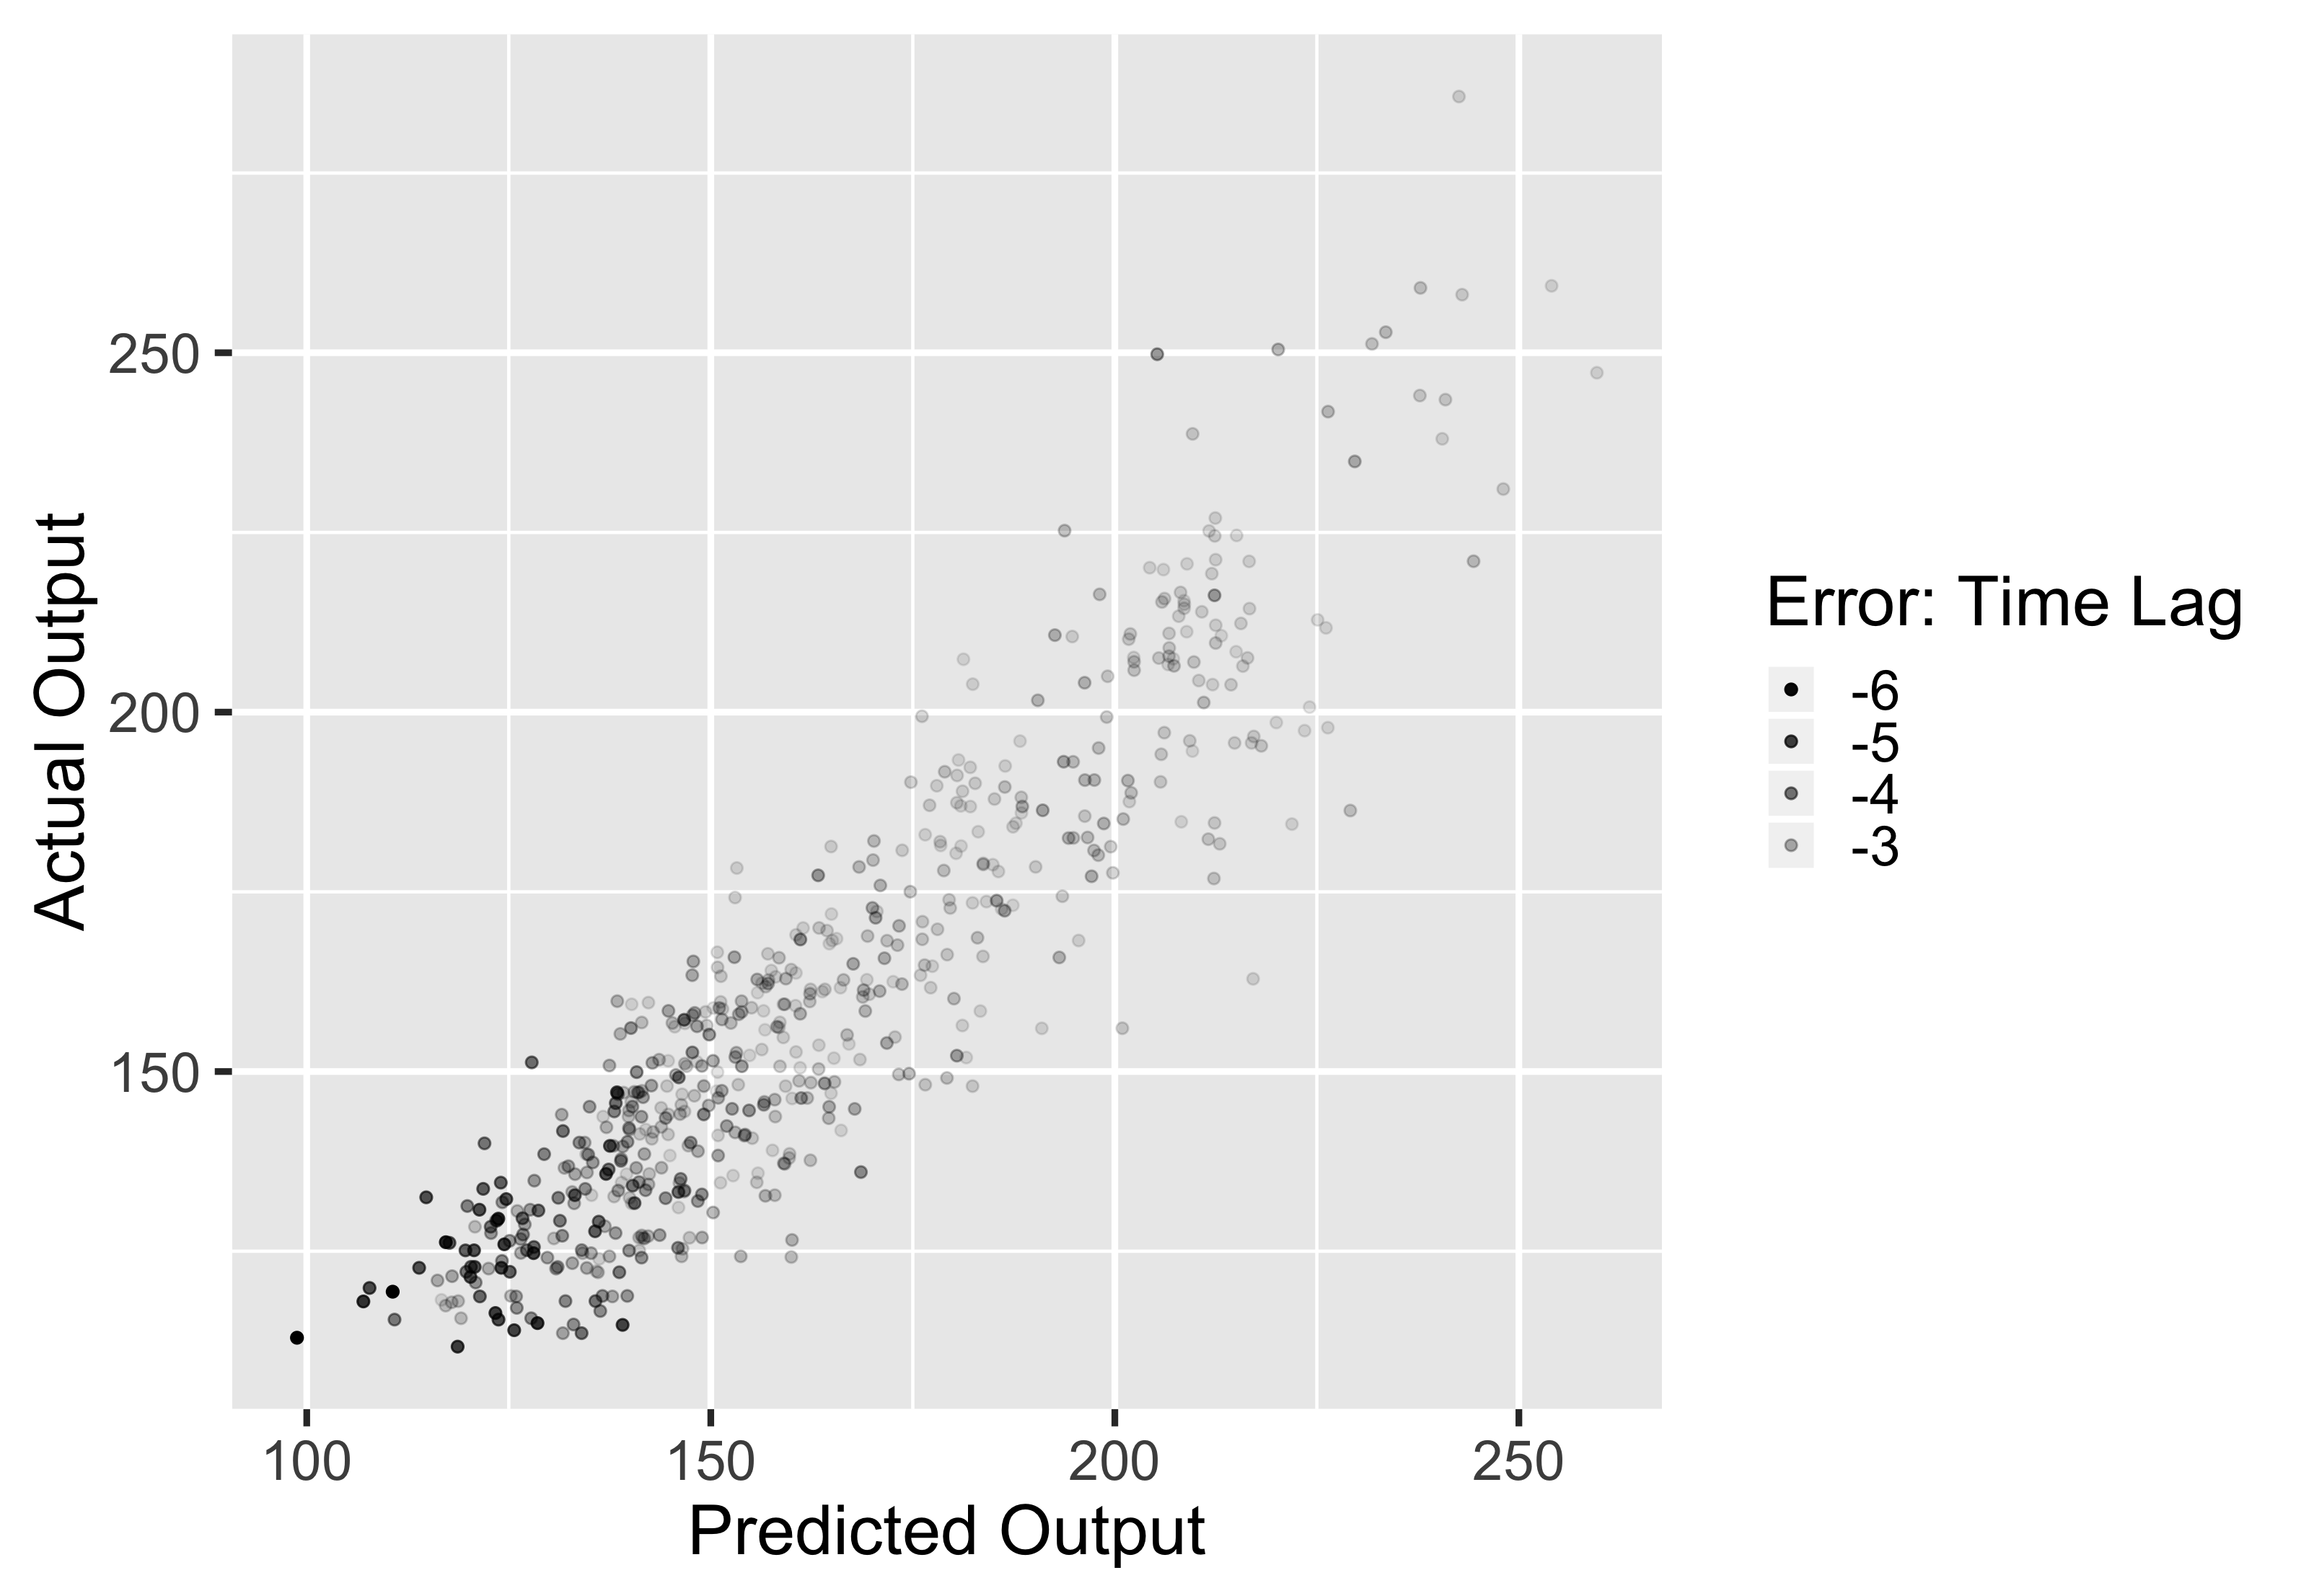
\includegraphics[width=0.5\textwidth]{figures/exp3_lag_error_jus.png}}
\vspace{.3in}
\caption{\textbf{Problem III}, Predicted vs Actual Outputs for the cases with time lag error $\leq -2.5$.}
\label{fig:problem3_lag_error_jus}
\end{figure}



\begin{table}[h]
\caption{\textbf{Problem III}: Statistics of the Output distribution} \label{table:problem3_stats}
\begin{center}
\begin{tabular}{ll}
\textbf{Statistic}  &\textbf{Value} \\
\hline \\
Minimum         & $111.7$ \\
$1$st Quartile  & $182.3$ \\
Median          & $252.1$ \\
$3$rd Quartile  & $334.5$ \\
Maximum         & $687.4$ \\
\end{tabular}
\end{center}
\end{table}


\subsubsection{Problem IV}

Figures \ref{fig:problem4_scatter}, \ref{fig:problem4_error}, \ref{fig:problem4_curves} summarize the results of the experiment. This case is different as compared to the previous problems as there is now
a monotonic relationship between the output and time lag. A key difference in the model performance in this problem can be observed in error scatter chart \ref{fig:problem4_error}, we can see that the time lag errors are symmetric.


\begin{figure}[h]
\vspace{.3in}
\centerline{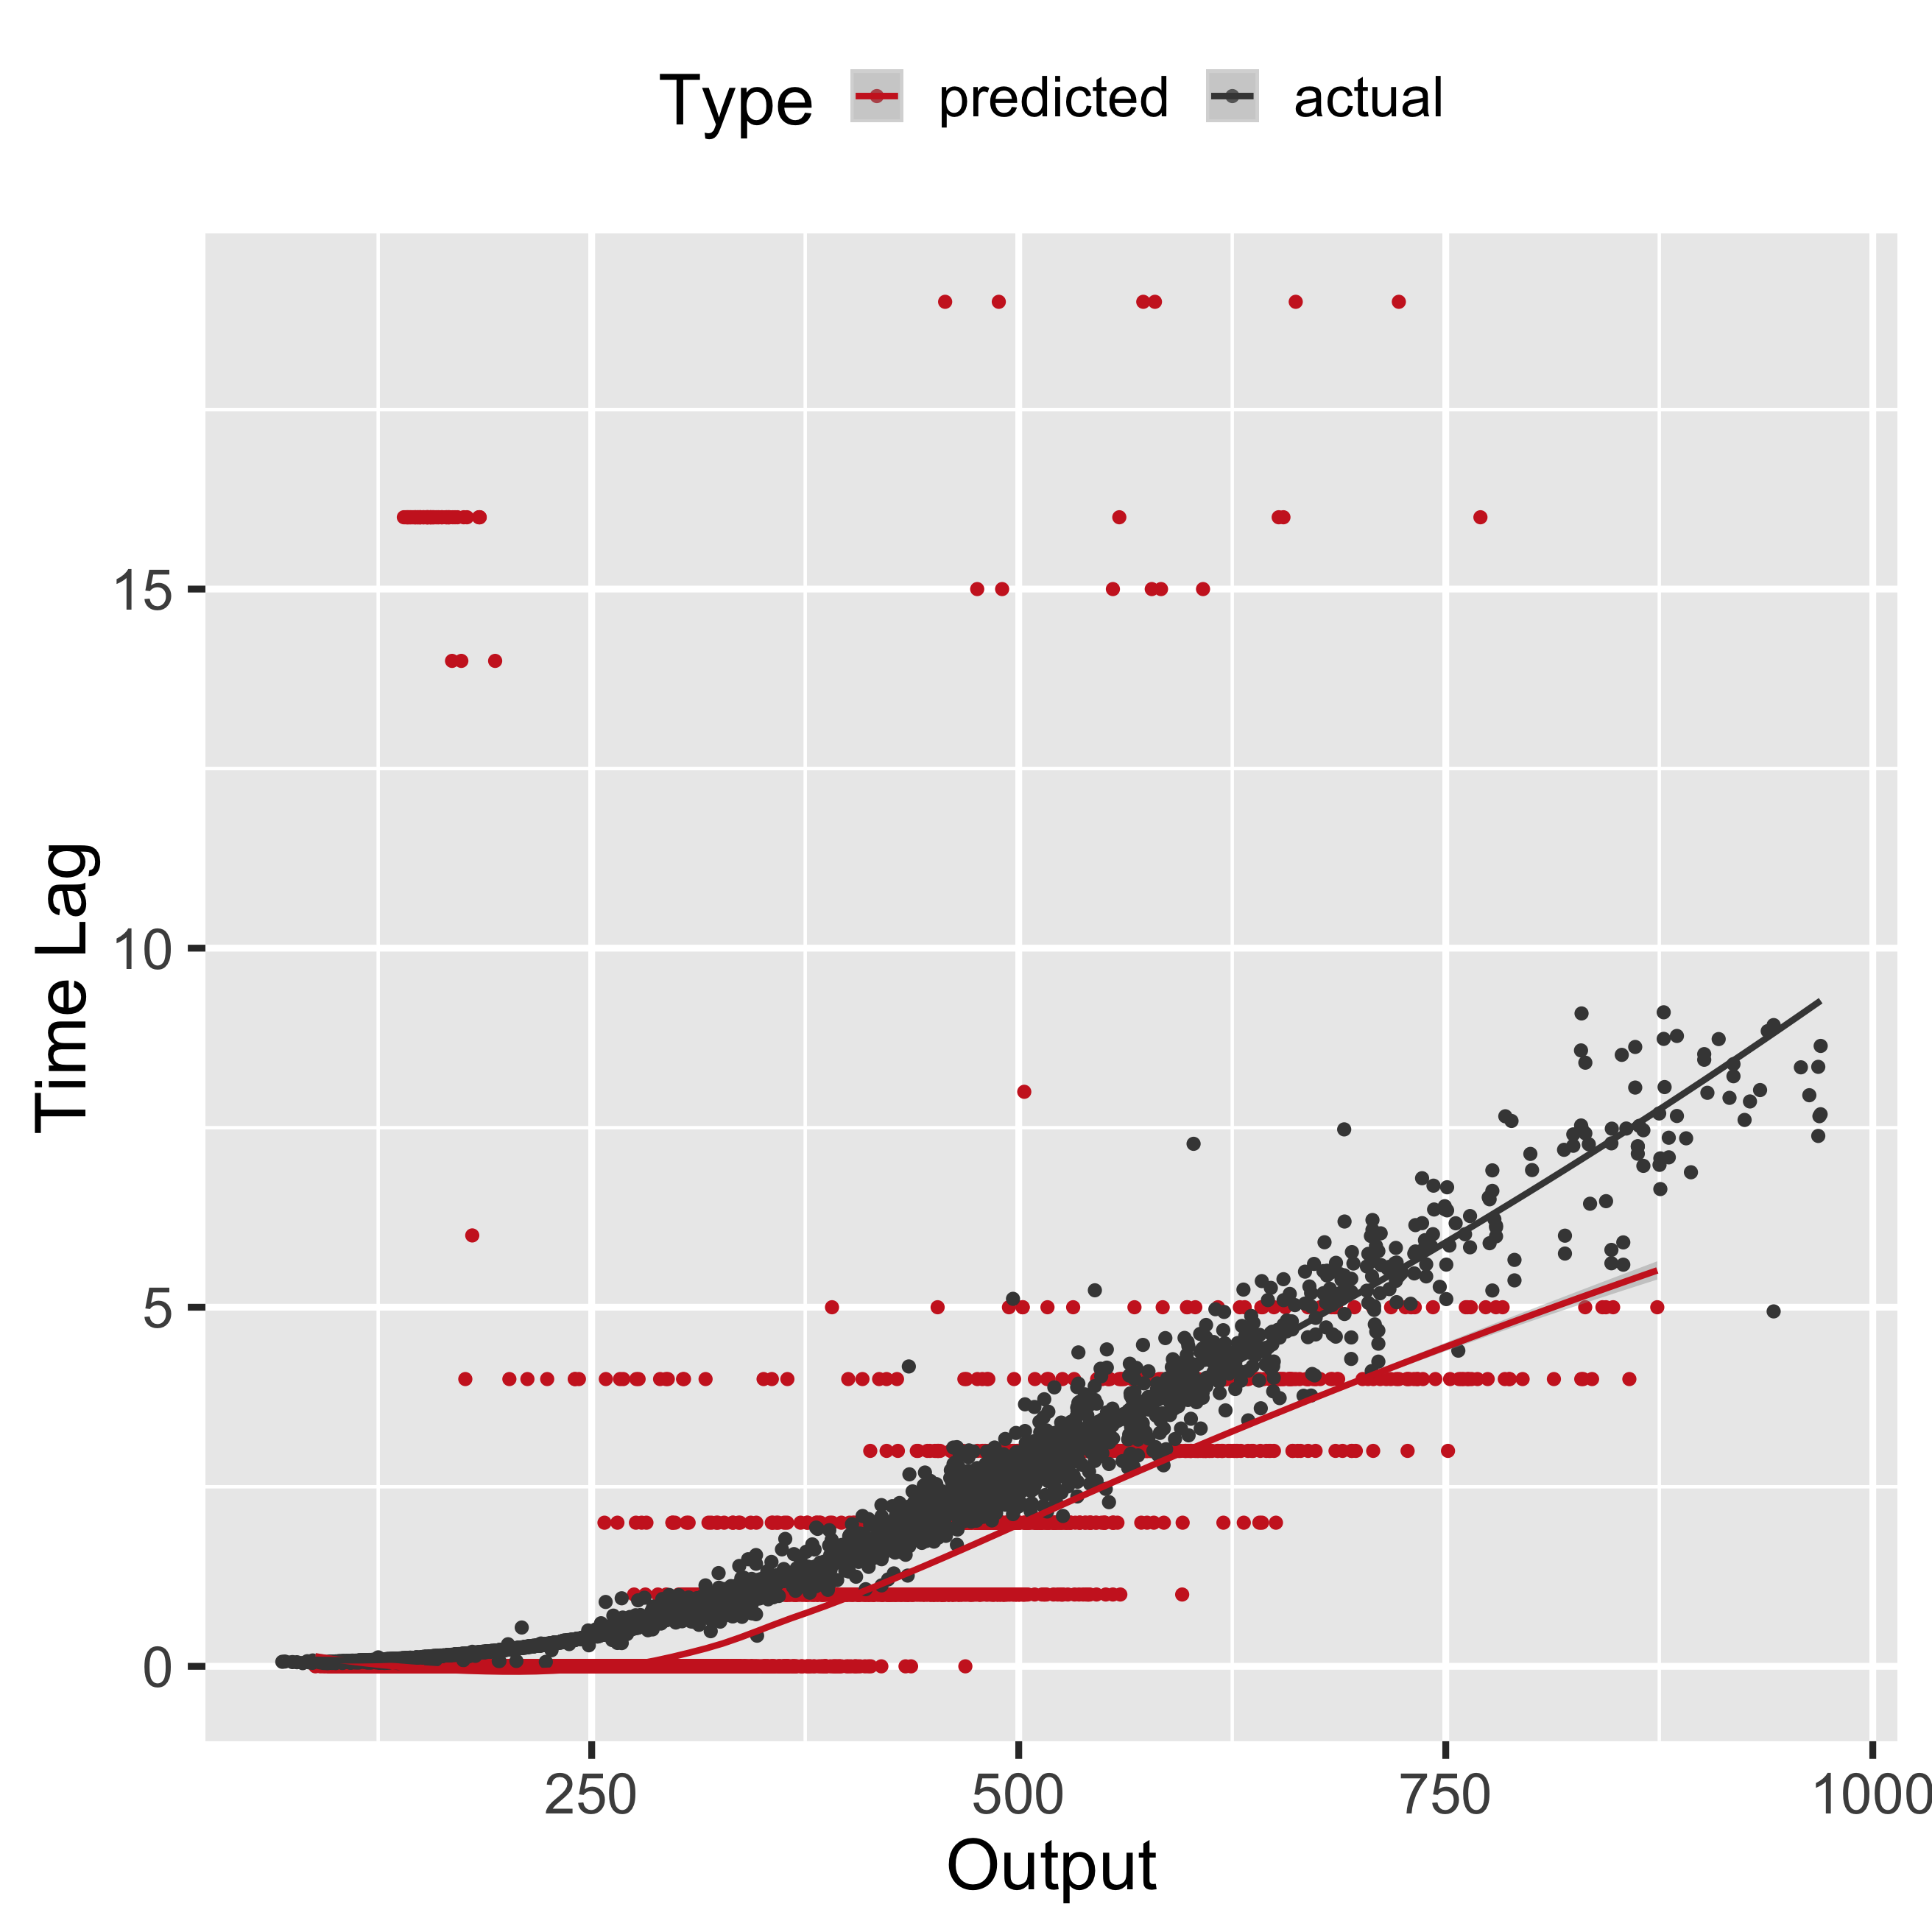
\includegraphics[width=0.5\textwidth]{figures/exp4_scatter_v_tl.png}}
\vspace{.3in}
\caption{\textbf{Problem IV}, Output-Time Lag Scatter plot; model predictions in red and actual data in black}
\label{fig:problem4_scatter}
\end{figure}

\begin{figure}[h]
\vspace{.3in}
\centerline{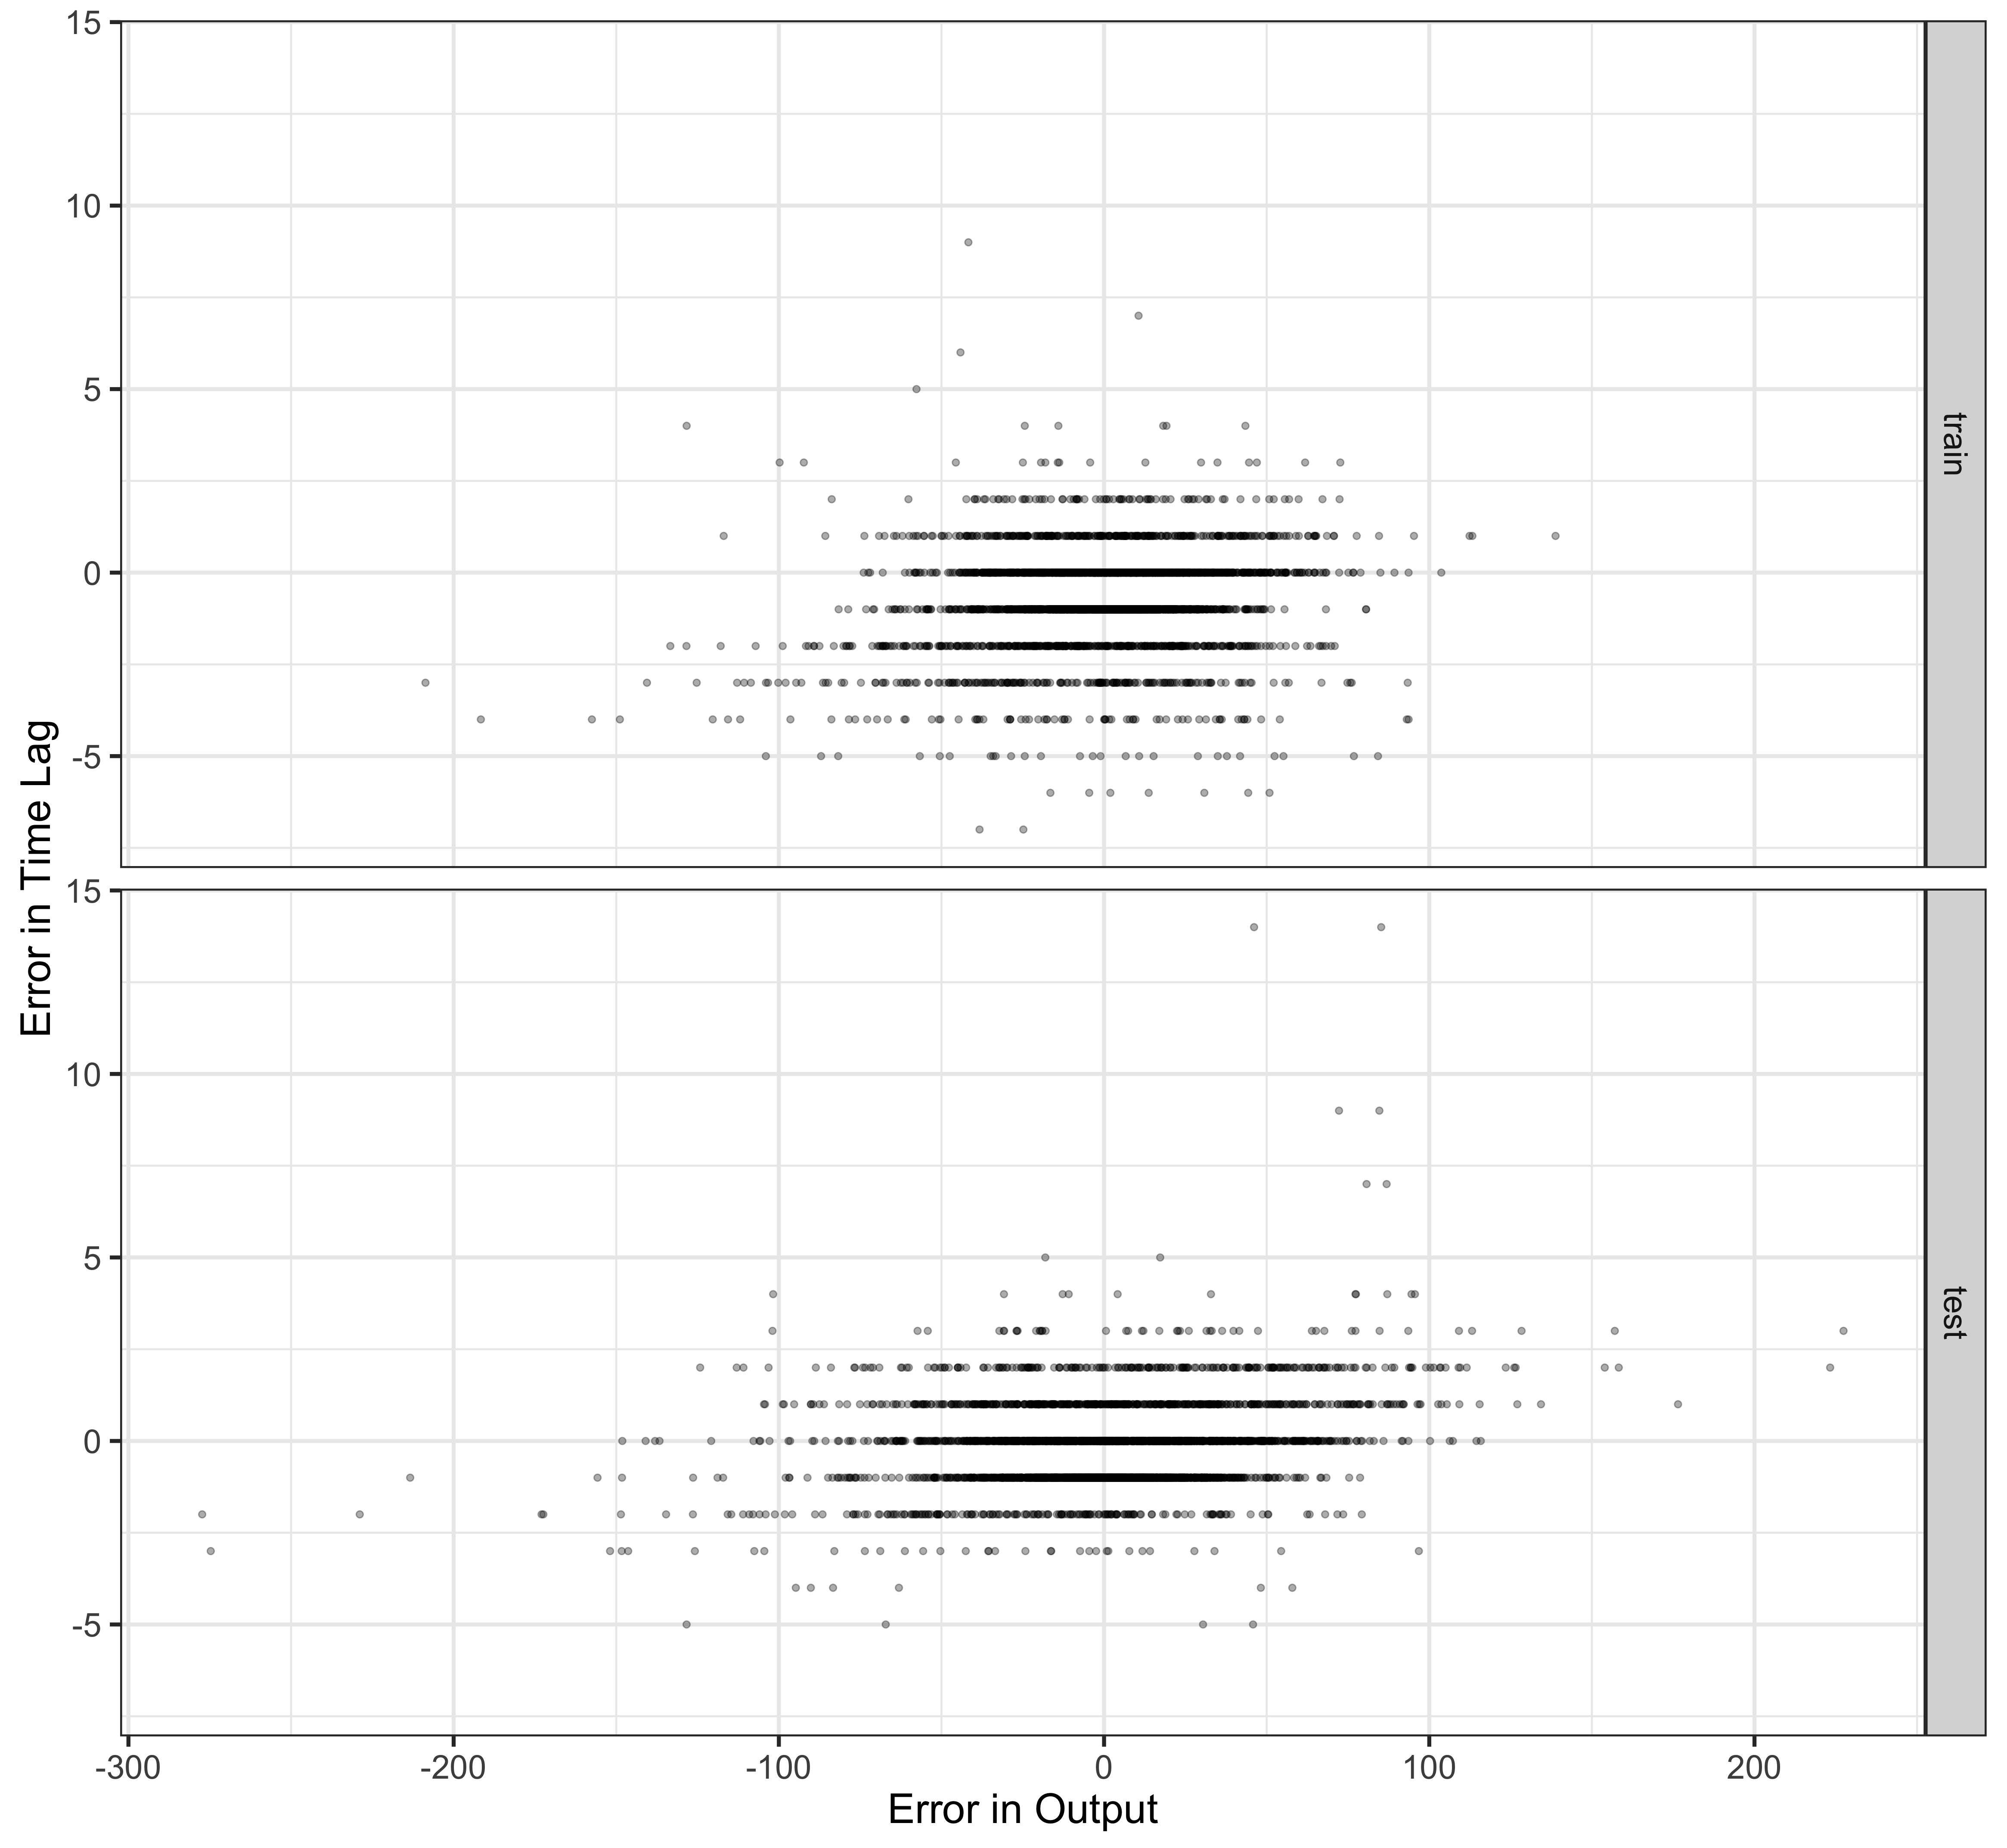
\includegraphics[width=0.5\textwidth]{figures/exp4_scatter_errors_test.png}}
\vspace{.3in}
\caption{\textbf{Problem IV}, Error in prediction of output vs error in time lag prediction}
\label{fig:problem4_error}
\end{figure}

\begin{figure}[h]
\vspace{.3in}
\centerline{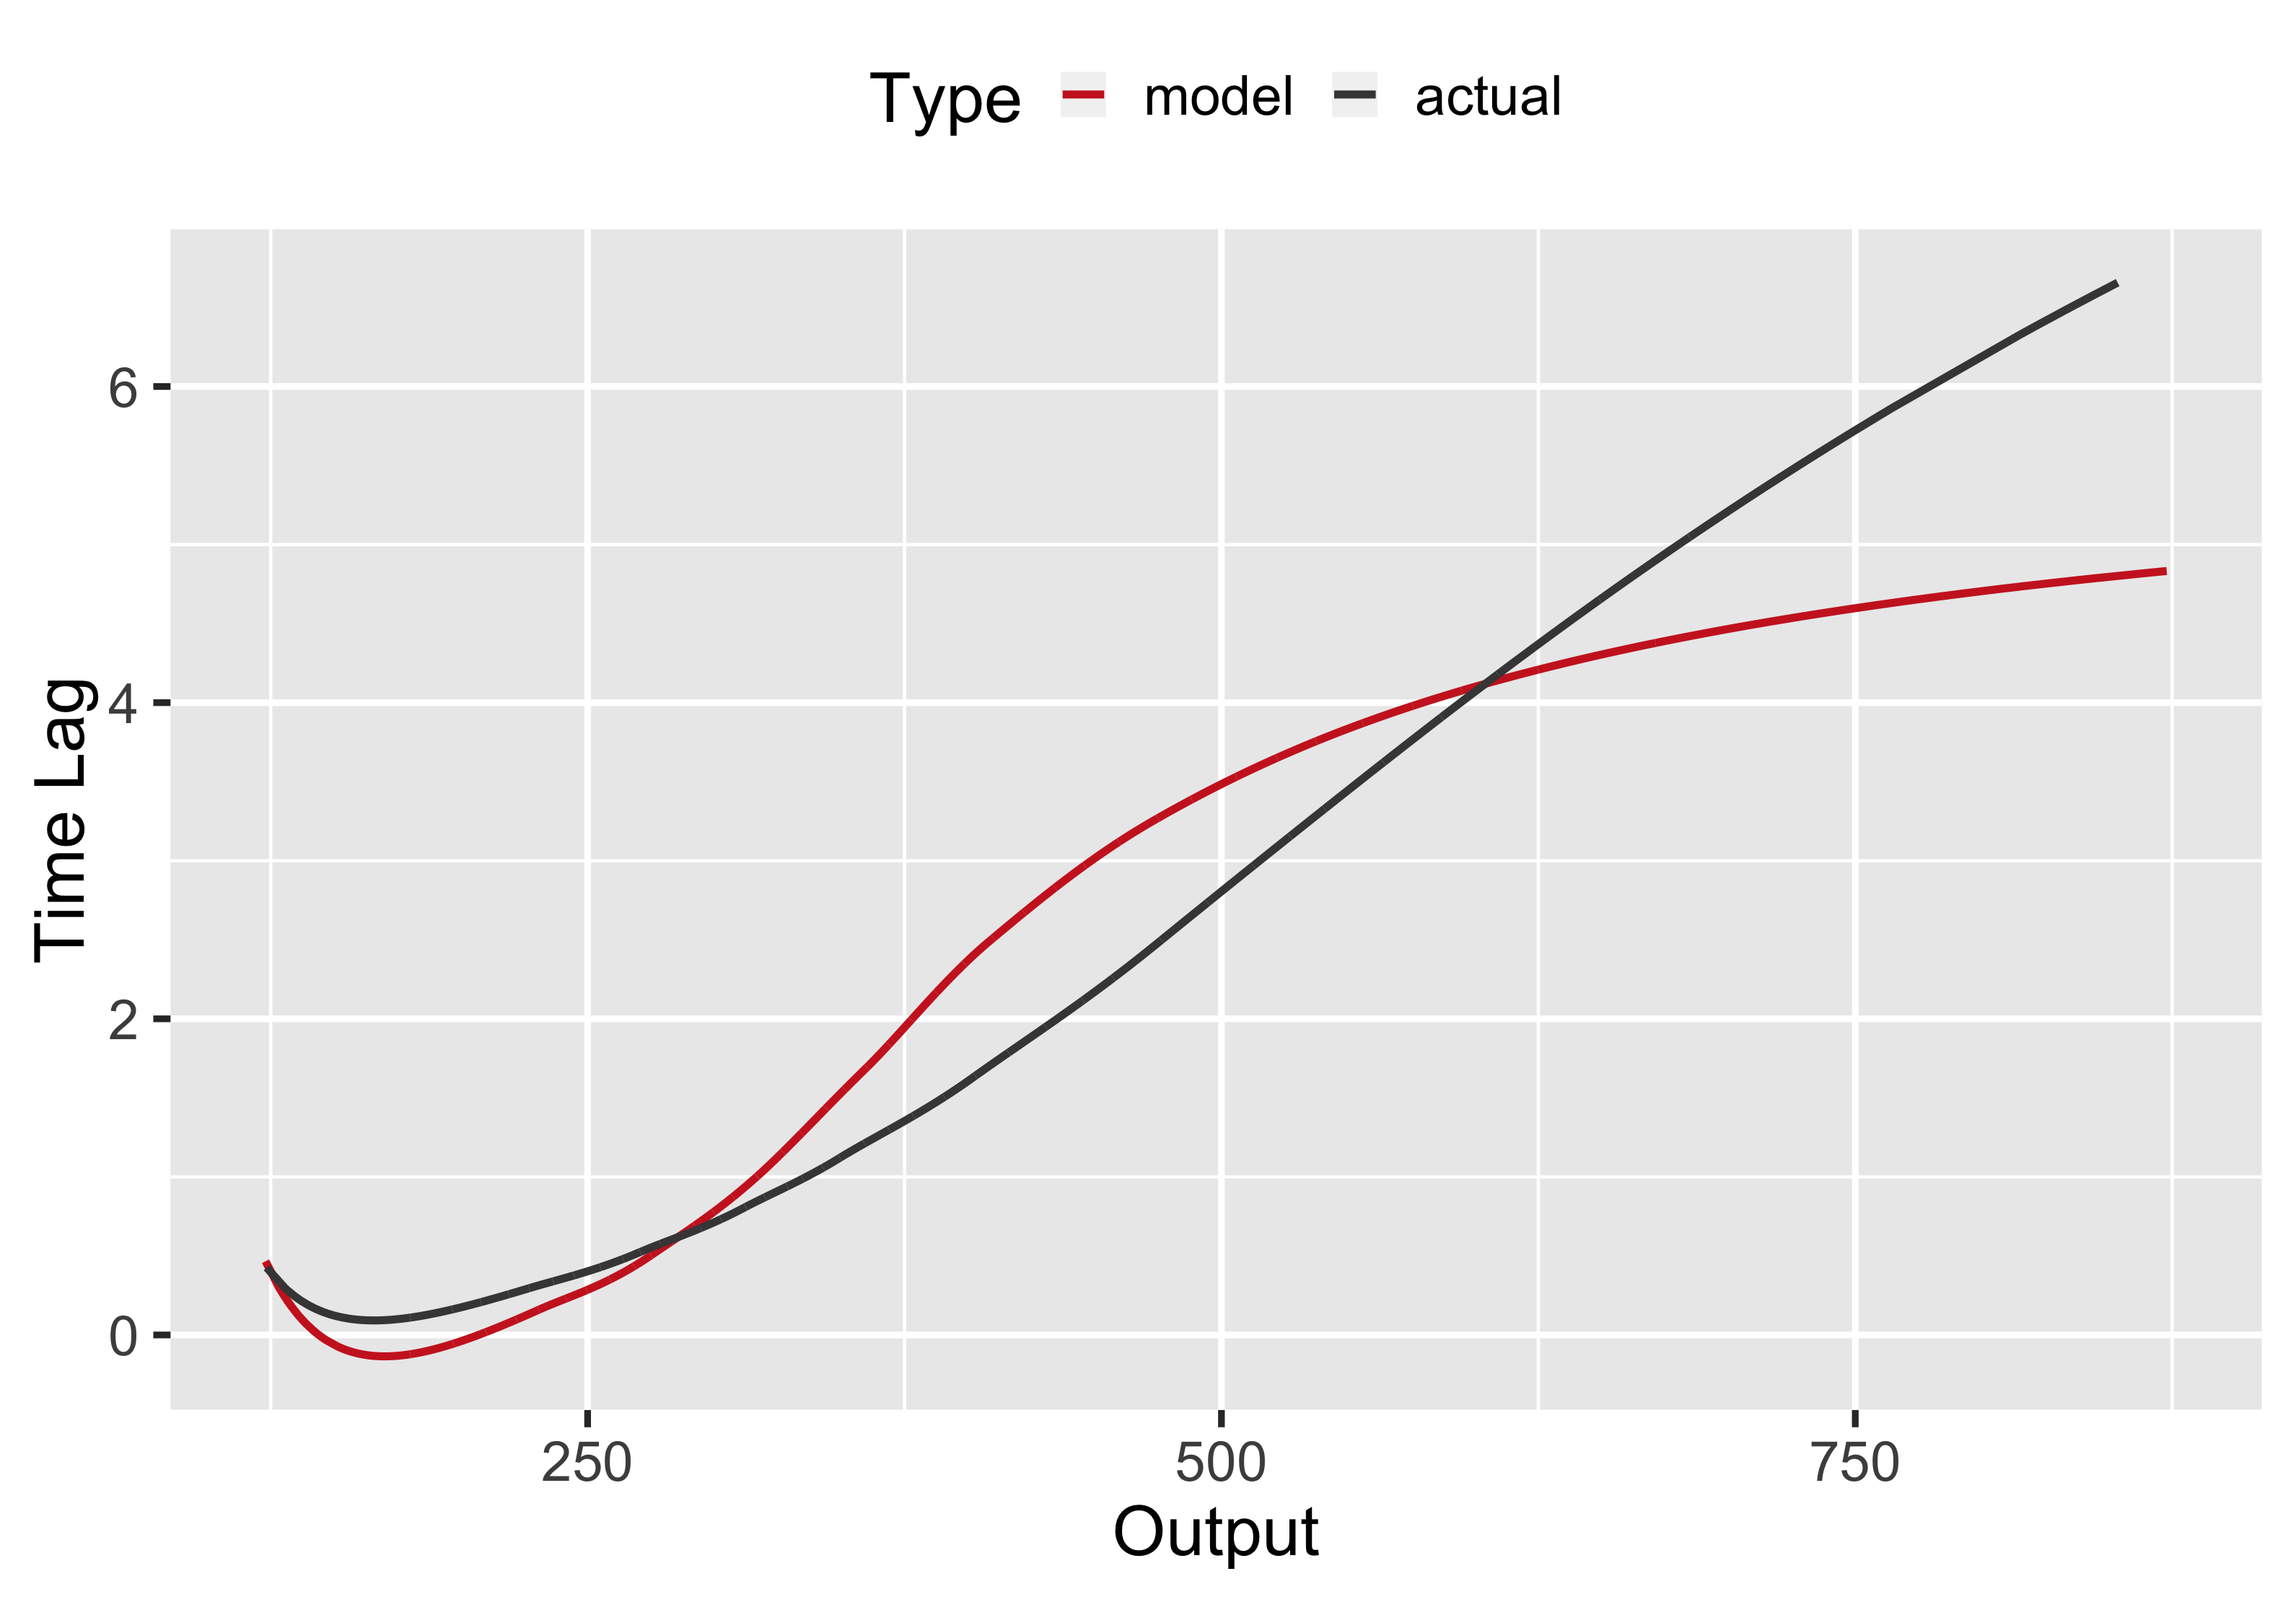
\includegraphics[width=0.5\textwidth]{figures/exp4_predictive_curves.png}}
\vspace{.3in}
\caption{\textbf{Problem IV}, Output vs Time Lag Relationship}
\label{fig:problem4_curves}
\end{figure}

\section{Conclusions}

We present in this work a formulation and a novel solution methodology for the problem of performing inference and forecasting in the context of lagged causal relationships between time series. We call this problem \emph{Causal Dynamic Time Lag} (CDT) to note the non-stationary nature of the causal link between time series $x(t)$ and $y(t)$. We outline a neural network based solution to this problem and benchmark its performance on a set of carefully constructed problems.

This work is an area of active research and progress. Going ahead we plan to apply this methodology to the problem of forecasting of geomagnetic phenomena which are driven by features observed on the surface of the Sun, i.e. sunspots and active regions.


\subsubsection*{Acknowledgements}

\bibliography{references}

\end{document}
